\documentclass[12pt,a4paper]{report}

\usepackage[a4paper,margin=1in]{geometry}
\usepackage{setspace}
\usepackage{graphicx}
\usepackage{amsmath}
\usepackage{amssymb}
\usepackage{booktabs}
\usepackage{titlesec}
\usepackage{cite}
\usepackage{placeins}
\usepackage{tikz}
\usepackage{multirow}
\usepackage{hyperref}
\usepackage{float}
\usetikzlibrary{calc, shapes.geometric, arrows, positioning}

\title{\textbf{Multi-Agent Deep Reinforcement Learning for Joint Service Caching and Computation Offloading in Vehicular Edge Computing}}
\author{Your Name}
\date{\today}

\doublespacing

\begin{document}

%========================================================
% TITLE PAGE
%========================================================
\begin{titlepage}
    \begin{center}
        \vspace*{1cm}
        
        \Large
        \textbf{Multi-Agent Deep Reinforcement Learning for Joint Service Caching and Computation Offloading in Vehicular Edge Computing}
        
        \vspace{1.5cm}
        
        \normalsize
        A Thesis Submitted in Partial Fulfillment of the Requirements \\
        for the Degree of \\
        \textbf{[Degree Name, e.g., Bachelor of Technology]}
        
        \vspace{1.5cm}
        
        \textbf{Submitted By:} \\
        \textbf{Your Name} \\
        \textbf{[Roll Number]}
        
        \vspace{1.5cm}
        
        \textbf{Under the Guidance of:} \\
        \textbf{[Supervisor Name]} \\
        \textbf{[Supervisor Designation]}
        
        \vfill
        
        \vspace{0.8cm}
        
        \Large
        \textbf{[Department Name]} \\
        \textbf{[University/College Name]} \\
        \textbf{[City, State, Zip Code]} \\
        \textbf{[Year]}
        
    \end{center}
\end{titlepage}

\newpage

\tableofcontents
\newpage

\listoffigures
\addcontentsline{toc}{chapter}{List of Figures}
\newpage

\listoftables
\addcontentsline{toc}{chapter}{List of Tables}
\newpage

%------------------------------------------------
\chapter*{Abstract}
\addcontentsline{toc}{chapter}{Abstract}

The rapid proliferation of smart vehicles and advanced vehicular applications, such as autonomous driving, augmented reality (AR) navigation, and real-time traffic monitoring, has generated an unprecedented demand for computational resources and ultra-low latency processing. Vehicular Edge Computing (VEC) has emerged as a transformative paradigm to address these stringent requirements by deploying computational and storage resources at the edge of the network, specifically at Roadside Units (RSUs). By bringing cloud-like capabilities closer to the data source, VEC enables vehicles to offload their computation-intensive tasks, thereby significantly reducing transmission latency and conserving the limited battery life of local vehicular devices. However, edge servers inherently possess limited computational and storage capacities compared to centralized core clouds. In realistic VEC scenarios, a computation task cannot be executed at the edge unless the corresponding service program is actively cached on that specific RSU. If the required service is missing from the RSU's cache, it must be fetched from the remote core cloud, incurring severe transmission delays that negate the benefits of edge computing. Therefore, to truly minimize system latency and energy consumption, computation offloading decisions must be jointly optimized with service caching strategies.\\

Traditional approaches to service caching rely on reactive heuristics such as Least Recently Used (LRU) and Least Frequently Used (LFU). While these methods are computationally lightweight, they perform poorly in highly dynamic Internet of Vehicles (IoV) environments because they fail to anticipate future vehicle trajectories or spatial-temporal task arrival patterns. Furthermore, while single-agent Deep Reinforcement Learning (DRL) models like Deep Deterministic Policy Gradient (DDPG) have shown promise in optimizing joint caching and offloading, they assume a stationary environment. This assumption breaks down in multi-vehicle scenarios, leading to "herding behavior"—where multiple independent vehicles simultaneously offload to the same RSU, causing sudden cache evictions, severe network congestion, and queue overloads. To overcome these critical limitations, a novel Multi-Agent Deep Reinforcement Learning (MARL) framework based on Multi-Agent Deep Deterministic Policy Gradient (MA-DDPG) for joint service caching and computation offloading in VEC environments is proposed.\\

The proposed framework utilizes a Centralized Training with Decentralized Execution (CTDE) architecture, supplemented by an explicit inter-agent communication protocol. During training, a centralized critic evaluates the joint actions and global state to guide the learning process, while during execution, local actors make decentralized decisions based on their local observations and continuous intent messages broadcasted by neighboring vehicles. This explicit communication mechanism enables vehicular agents to proactively negotiate caching intents, resolve resource conflicts, and maintain optimal cache diversity across the network. The framework handles the highly dynamic mobility of vehicles by processing spatial-temporal state representations, ensuring that offloading and caching decisions are continuously adapted to the changing environment.\\

The proposed framework is rigorously evaluated using a custom VEC simulator built upon the LEAF framework and integrated with realistic urban mobility traces generated by the SUMO traffic simulator. Experimental analysis is conducted under varying parameters, including vehicle density, task sizes, and edge server cycle frequencies. The performance of the MA-DDPG framework is compared against state-of-the-art baselines, including single-agent DDPG, Latency Minimization, Energy Minimization, LRU edge caching, and a No-Cache scheme. Results demonstrate that the proposed MA-DDPG model significantly outperforms all baseline methods, achieving the lowest total system cost. Ablation studies further confirm the effectiveness of the communication protocol and the CTDE architecture in enhancing model performance and stability. Overall, the proposed framework achieves a superior balance between computation efficiency, latency reduction, and network scalability for secure and efficient resource management in next-generation Vehicular Edge Computing networks.\\

\noindent
\textbf{Keywords :} Vehicular Edge Computing (VEC), Multi-Agent Reinforcement Learning (MARL), Deep Deterministic Policy Gradient (DDPG), Service Caching, Computation Offloading, CTDE Architecture, Internet of Vehicles (IoV).

\newpage

%------------------------------------------------
\chapter{Introduction}

The landscape of modern transportation is undergoing a paradigm shift driven by the evolution of 5G and emerging 6G wireless communication networks, leading to the realization of the Internet of Vehicles (IoV). Smart vehicles today are no longer merely mechanical modes of transport; they are highly sophisticated computing platforms equipped with a multitude of sensors, cameras, RADARs, and LiDARs. These vehicles run advanced, computation-intensive applications such as autonomous driving algorithms, Augmented Reality (AR) assisted navigation, real-time traffic condition monitoring, high-definition video streaming, and sophisticated infotainment systems. These applications demand massive computational resources and impose stringent requirements on ultra-low latency to ensure passenger safety and provide a seamless user experience. Efficient management of computational resources is essential to ensure better Quality of Service (QoS), reduced operational costs, lower energy consumption, and improved overall system performance \cite{vec_concept}.Vehicular Edge Computing (VEC) environments are highly dynamic because computational workloads continuously change depending on vehicle mobility and traffic density. Resource utilization at Roadside Units (RSUs) may vary significantly over time due to fluctuations in task offloading requests and edge-level scheduling operations. In such environments, accurate prediction and allocation of edge resources becomes an important task. Predicting future CPU, memory, and cache usage enables VEC providers to allocate resources proactively, avoid resource bottlenecks, minimize transmission latency, and improve infrastructure utilization. Accurate caching and offloading predictions also help reduce under-utilization and over-utilization of edge servers, which directly impacts energy efficiency and operational cost \cite{mobility_caching}.\\

Traditional resource allocation methods generally rely on real-time information without considering future mobility patterns. As a result, these methods often fail to make optimal resource provisioning decisions in highly heterogeneous VEC environments. Machine learning and deep learning approaches have recently shown significant improvements in workload prediction and resource allocation by learning complex patterns from historical mobility traces. Models such as Deep Q-Networks (DQN) and Deep Deterministic Policy Gradient (DDPG) are increasingly used for edge resource prediction because of their ability to model nonlinear relationships and temporal dependencies in large-scale vehicular datasets \cite{joint_caching_offloading}.Among these approaches, Multi-Agent Reinforcement Learning (MARL) has emerged as a promising distributed learning paradigm that enables multiple vehicular clients to collaboratively learn an optimal joint policy. Instead of relying on a single centralized controller which introduces massive communication overhead, vehicular agents learn continuous offloading and caching strategies locally, significantly improving scalability and reducing the risks associated with centralized decision bottlenecks \cite{maddpg_paper}.\\

Despite the advantages of MARL, several challenges still exist in practical VEC environments. One of the major issues is the presence of non-stationary environments across different agents, where the actions of one vehicle directly alter the state observed by others. Such non-stationarity can reduce model convergence speed and policy stability. In addition, recent studies have shown that independent agents operating without coordination often engage in "herding behavior", where multiple vehicles simultaneously target the same RSU, causing severe cache thrashing and network congestion. Centralized Training with Decentralized Execution (CTDE) has been widely adopted to address these non-stationarity concerns by utilizing a global critic during training. However, without explicit inter-agent communication, actors may still execute conflicting actions during deployment \cite{marl_comm}. Therefore, designing an efficient multi-agent framework that achieves a better balance between decentralized execution and explicit intent coordination remains an important research challenge in VEC resource optimization.

\section{Scope of Project}
The scope of this project is to develop a communication-enhanced MARL framework for accurate joint service caching and computation offloading in Vehicular Edge Computing environments. The proposed system predicts optimal offloading destinations and proactive caching replacements while ensuring that multi-agent resource conflicts are minimized. The project focuses on integrating the Multi-Agent Deep Deterministic Policy Gradient (MA-DDPG) algorithm with a Centralized Training, Decentralized Execution (CTDE) architecture. A continuous intent-sharing communication protocol is introduced to resolve resource conflicts and prevent herding behavior among independent vehicular agents. The proposed framework handles highly dynamic mobility traces using SUMO and the LEAF edge computing simulator. The system is evaluated under varying vehicle densities, task sizes, and computational capacities, and compared with existing methods such as single-agent DDPG, LRU, and greedy heuristics to validate its superiority in minimizing latency and energy consumption.

\section{Applications}

\begin{itemize}

\item \textbf{Autonomous Driving Navigation:}  
The proposed system facilitates real-time processing of massive sensor data by ensuring that necessary machine learning models (e.g., object detection, trajectory prediction) are cached at the edge, guaranteeing the ultra-low latency required for safe autonomous navigation.

\item \textbf{Augmented Reality (AR) Assisted Driving:}  
The framework enables immersive AR navigation systems on vehicle windshields by intelligently offloading heavy rendering tasks to edge servers that cache the required AR rendering engines and local high-definition map data.

\item \textbf{Smart Traffic Flow Optimization:}  
Processing aggregated traffic data from multiple vehicles at the edge to provide real-time route optimization, hazard warnings, and traffic light scheduling without relying on distant cloud servers, drastically reducing response times.

\item \textbf{In-Vehicle Infotainment Systems:}  
The proposed model improves the Quality of Experience (QoE) for passengers by providing low-latency access to media transcoding services, gaming servers, and high-definition video streaming cached directly at RSUs.

\item \textbf{Energy-Efficient Edge Resource Management:}  
Accurate caching and offloading predictions minimize unnecessary data transmissions to the core cloud and prevent RSU overloads. This reduces power consumption across the network and improves overall energy efficiency.

\item \textbf{Cooperative Distributed Computing Grids:}  
Integrating with broader smart city initiatives by turning vehicles and RSUs into a cooperative, distributed computing grid capable of handling localized data processing tasks efficiently, resolving conflicts through continuous multi-agent communication.

\item \textbf{Dynamic Resource Scaling in RSUs:}  
The framework supports automatic scaling of computation offloading ratios based on current RSU workload demand. During peak traffic conditions, tasks can be intelligently distributed to the cloud to maintain performance and prevent edge crashes.

\item \textbf{Quality of Service (QoS) Improvement for V2X:}  
The proposed model helps prevent edge system overload and bandwidth bottlenecks through proactive caching negotiation. This improves response time, reliability, and service availability for all connected vehicles.

\item \textbf{Real-Time Video Surveillance and Analytics:}  
Joint caching allows heavy computer vision models to reside at the edge, enabling rapid processing of dashboard camera feeds for real-time anomaly detection and surveillance without overwhelming the core network.

\item \textbf{Secure Multi-Agent Edge Environments:}  
The CTDE architecture provides a foundation for secure multi-agent coordination where vehicles do not need to share their raw internal states during execution, reducing communication overhead and enhancing scalability in dense deployments.

\end{itemize}
%------------------------------------------------

\chapter{Motivation}

The increasing dependence on connected and autonomous vehicles has created a strong demand for intelligent and efficient resource management systems at the network edge. Modern IoV platforms host a multitude of applications related to artificial intelligence, online streaming, sensor fusion, and real-time analytics. These applications continuously generate highly dynamic workloads that consume CPU, memory, and bandwidth resources at varying rates. Managing such rapidly changing workloads efficiently is a major challenge for network providers because improper allocation of edge resources can directly affect system performance, operational cost, and most critically, passenger safety. One of the primary reasons for this project is the inefficiency of traditional edge resource allocation methods. In many VEC infrastructures, caching decisions are made reactively using heuristics such as Least Recently Used (LRU) or Least Frequently Used (LFU). Such approaches are insufficient in dynamic environments because they fail to anticipate future resource demands and vehicle mobility patterns. When future caching needs are not predicted accurately, edge systems experience high cache miss rates, forcing tasks to be routed to the distant core cloud. This causes resource bottlenecks, increased transmission latency, and degraded Quality of Service (QoS). On the other hand, static offloading strategies fail to adapt to the real-time computational load of RSUs. Therefore, intelligent, joint optimization of caching and offloading has become an essential requirement for modern IoV systems.\\

The limitations of single-agent reinforcement learning present another significant concern addressed in this work. While Deep Reinforcement Learning (DRL) has been widely adopted for resource allocation, standard models like Deep Deterministic Policy Gradient (DDPG) assume a stationary environment or a single centralized controller. In real-world vehicular networks, multiple independent vehicles (agents) interact with the same shared edge resources simultaneously. When multiple vehicles employ independent DRL agents without coordination, it leads to a non-stationary environment. An action taken by one vehicle (e.g., filling an RSU's cache) directly alters the state observed by another vehicle. This non-stationarity causes severe instability during training and leads to suboptimal, greedy decisions. Multi-Agent Reinforcement Learning (MARL) emerged as a potential solution to these coordination concerns because it enables collaborative policy learning. However, practical deployment of MARL in dense vehicular environments still faces several unresolved challenges that motivated this research work.\\

One of the major problems in MARL is the presence of uncoordinated "herding behavior". In real-world VEC systems, if a particular RSU is observed to have available cache space and low computational load, multiple uncoordinated agents may simultaneously decide to offload their tasks to that RSU and request it to cache their specific services. This simultaneous influx overwhelms the RSU's queue and triggers a cascade of cache evictions, severely degrading prediction accuracy and system stability. Traditional multi-agent algorithms struggle to handle such conflicts because local actors often execute identical actions based on identical local observations. This results in unstable execution, slower convergence, and reduced task success rates. The problem becomes even more critical when strict latency requirements are introduced. Existing DDPG-based methods often use continuous action spaces without considering the quality or stability of simultaneous caching updates. As a result, unnecessary conflicts are introduced into the edge queue, reducing prediction performance and slowing convergence. This created the need for a more intelligent intent-sharing mechanism capable of balancing decentralized execution and cooperative intent dynamically.\\

Another major challenge comes from the limitations of existing multi-agent approaches such as independent DDPG and standard CTDE. Independent DDPG attempts to handle multi-agent scenarios, but its performance degrades rapidly as the number of vehicles increases because non-stationarity weakens model learning. Similarly, standard CTDE introduces a global critic to stabilize training. However, static decentralized actors without communication still lead to execution-time instability and resource thrashing when faced with identically optimal edge nodes.\\

These limitations motivated the development of a new framework that could:
\begin{itemize}
    \item Improve joint caching and offloading accuracy in highly dynamic IoV environments.
    \item Resolve the non-stationarity problem inherent in multi-agent reinforcement learning.
    \item Prevent "herding behavior" and catastrophic cache thrashing at RSUs.
    \item Improve model convergence and training stability through centralized training.
    \item Support scalable, decentralized execution enhanced by explicit communication protocols.
\end{itemize}

The introduction of an explicit intent-sharing communication protocol in this project helps overcome the limitations of uncoordinated MARL. Instead of acting blindly, the proposed approach dynamically adjusts caching requests based on continuous message vectors broadcasted by neighboring vehicles. Agents contributing identical requests negotiate to select diverse caching targets. This adaptive mechanism helps achieve a better latency-efficiency trade-off without sacrificing decentralized execution speed. Similarly, Centralized Training with Decentralized Execution (CTDE) helps reduce conflicts caused by non-stationary environment dynamics. By evaluating joint actions globally during training, the network's value approximations become more coherent and stable. Dynamic intent sharing further improves adaptability because vehicle density and edge availability change continuously over time. This makes static MARL execution insufficient for real-world applications.\\

Experimental evaluation using the LEAF simulator and realistic SUMO mobility traces further supports this work by demonstrating that existing approaches still suffer from significant prediction errors and instability under dense conditions. The proposed MA-DDPG framework with continuous intent sharing and CTDE architecture aims to overcome these challenges by combining accurate continuous learning with intelligent multi-agent conflict resolution mechanisms.

%------------------------------------------------
\chapter{Literature Survey}

\section{Prediction methods for effective resource provisioning in cloud computing: A survey}
K. Dinesh Kumar and E. Umamaheswari presented a comprehensive survey on prediction methods for effective resource provisioning in cloud computing environments. The paper analyzed various machine learning and statistical prediction techniques for workload forecasting and dynamic resource allocation. The study highlighted the importance of accurate prediction methods in improving QoS, reducing SLA violations, optimizing energy consumption, and enhancing cloud and edge resource utilization efficiency.

\section{Computation Offloading and Content Caching for MEC in Software Defined Vehicular Networks}
Zhao et al. investigated the joint optimization of computation offloading and content caching in Vehicular Edge Computing environments utilizing Software Defined Networking (SDN). The paper formulated the problem as a mixed-integer non-linear programming (MINLP) model to minimize the total latency of vehicular tasks. The authors proposed a collaborative caching scheme where RSUs share their cached contents to improve the overall cache hit rate. While their mathematical approach provided optimal solutions under static conditions, the heavy computational complexity of MINLP makes it unsuitable for real-time decision-making in highly dynamic, fast-moving vehicular networks where network topologies change every few seconds.

\section{Deep Reinforcement Learning for Joint Caching and Offloading in VEC}
Zhang et al. proposed a single-agent Deep Reinforcement Learning framework to tackle the joint caching and offloading problem. By utilizing the Deep Deterministic Policy Gradient (DDPG) algorithm, the framework learned to make continuous offloading and caching replacement decisions by interacting with the environment, entirely bypassing the need for computationally expensive MINLP solvers. The study demonstrated that DRL could significantly reduce system delay compared to traditional heuristics like LRU. However, the model assumed a single centralized agent controlling all vehicles, which introduces massive communication overhead and scalability issues as the number of vehicles increases.

\section{Multi-Agent Actor-Critic for Mixed Cooperative-Competitive Environments}
Lowe et al. introduced the Multi-Agent Deep Deterministic Policy Gradient (MA-DDPG) algorithm, extending traditional actor-critic methods to multi-agent environments. The paper proposed the Centralized Training, Decentralized Execution (CTDE) architecture, which utilizes a centralized critic to observe the global state and joint actions during training to stabilize learning, while decentralized actors take actions based only on local observations during execution. The study demonstrated that MA-DDPG effectively overcomes the non-stationarity problem inherent in independent Q-learning or DDPG. Their work provided the foundational theoretical framework for applying MARL to complex, distributed resource allocation problems.

\section{Learning Multiagent Communication with Backpropagation}
Sukhbaatar et al. explored the necessity of communication in multi-agent reinforcement learning. They proposed CommNet, a continuous communication protocol where agents output a continuous message vector alongside their action. These messages are pooled and fed into the hidden layers of other agents at the next time step, allowing for backpropagation through the communication channel. The study showed that agents could learn to negotiate and cooperate explicitly, significantly improving performance in fully cooperative tasks compared to agents operating in silence. This highlighted the importance of intent sharing in resolving conflicts in shared environments.

\section{Mobility-Aware Edge Caching in Vehicular Networks using Deep Learning}
Li et al. addressed the challenge of high-speed vehicle mobility in VEC caching. They proposed a mobility-aware proactive caching strategy that utilizes recurrent neural networks (LSTMs) to predict vehicle trajectories based on historical SUMO traces. By predicting which RSU a vehicle will connect to in the near future, the system can proactively cache the required services at the target RSU before the vehicle arrives, minimizing cache misses. While effective at handling mobility, the study treated caching in isolation and did not jointly optimize it with the continuous, real-time computation offloading decisions required for delay-sensitive tasks.

\section{Resource Allocation in VEC using Heuristic Approaches}
Kumar et al. presented a comprehensive survey on traditional heuristic and statistical prediction methods for effective resource provisioning in edge computing. The paper analyzed reactive caching strategies such as Least Recently Used (LRU) and Least Frequently Used (LFU), as well as greedy offloading strategies based on latency minimization (LatencyMin) and energy minimization (EnergyMin). The survey highlighted that while heuristics are computationally inexpensive and easy to deploy, they consistently lead to suboptimal resource utilization and frequent QoS violations in highly dynamic environments because they completely lack the ability to anticipate future network states or workload patterns.

\section{Deep Reinforcement Learning for Resource Allocation in V2V Communications}
Ye et al. proposed a decentralized resource allocation mechanism for Vehicle-to-Vehicle (V2V) communications based on deep reinforcement learning. The paper demonstrated how independent agents could learn to select optimal sub-bands and power levels to maximize V2V link capacity while meeting strict latency constraints. The study highlighted the challenges of multi-agent environments, showing that while independent DRL can operate decentrally, it suffers from severe convergence instability compared to coordinated approaches.

\section{Multi-Agent Reinforcement Learning for Cooperative Edge Caching}
Jiang et al. proposed a cooperative edge caching framework utilizing multi-agent reinforcement learning to optimize cache hit rates across multiple base stations. The study modeled the base stations as independent agents attempting to learn a joint caching policy. The paper demonstrated that enabling explicit state sharing between agents significantly improved the global cache hit ratio and reduced overall transmission delay compared to isolated caching strategies like LRU or LFU, proving the necessity of inter-agent coordination in distributed edge networks.

%------------------------------------------------
\chapter{Problem Statement and Objectives}

\section{Problem Statement}

Existing methods such as independent single-agent Deep Deterministic Policy Gradient (DDPG), Least Recently Used (LRU) caching, and greedy latency heuristics experience uncoordinated action conflicts, execution instability, and poor robustness, leading to reduced efficiency in minimizing latency and energy consumption during joint service caching and computation offloading in highly dynamic vehicular edge computing environments.

%------------------------------------------------

\section{Objectives}

The main objectives of this project are:

\begin{itemize}

\item To develop a communication-enhanced Multi-Agent Reinforcement Learning (MARL) framework for Vehicular Edge Computing resource management.

\item To predict optimal offloading destinations and proactive service caching replacements using continuous action spaces accurately.

\item To implement a Multi-Agent Deep Deterministic Policy Gradient (MA-DDPG) algorithm for modeling structural and temporal workload relationships.

\item To preserve cache diversity by integrating explicit continuous intent-sharing protocols between vehicular agents.

\item To design a stability-aware Centralized Training, Decentralized Execution (CTDE) mechanism to improve learning stability.

\item To handle heterogeneous non-stationary multi-agent dynamics using shared global critics during training.

\item To improve global model convergence and mitigate catastrophic "herding behavior" and cache thrashing at RSUs.

\item To evaluate the robustness of the proposed framework under dynamic mobility constraints utilizing SUMO traffic traces and LEAF.

\item To compare the proposed model with existing approaches such as NoCache, LRU, LatencyMin, EnergyMin, and DDPG using performance metrics including Total Delay and Total Energy.

\item To analyze the performance of the proposed multi-agent framework under different operational parameters such as varying vehicle densities ($\rho$), task data sizes, and edge server CPU cycle frequencies.

\end{itemize}

%------------------------------------------------
\chapter{Methodology}
\label{ch:methodology}

\section{Road Network Data Collection}
The study started with collecting the real-world road network from the Surathkal region using OpenStreetMap (OSM).
The OSM Web Wizard available in SUMO was used to download:
\begin{itemize}
    \item Road network
    \item Junctions
    \item Lane information
    \item Vehicle routes
    \item Traffic movement data
\end{itemize}
The downloaded network was converted into SUMO-compatible files.
Generated files include:
\begin{itemize}
    \item osm.net.xml.gz
    \item osm.passenger.trips.xml
    \item osm.sumocfg
    \item osm.view.xml
\end{itemize}

\section{SUMO Traffic Simulation}
After generating the road network, traffic simulation was performed using SUMO (Simulation of Urban Mobility).
The simulation was executed using the following command:
\begin{verbatim}
sumo -c osm.sumocfg
\end{verbatim}
The simulator generated realistic vehicular mobility behavior including:
\begin{itemize}
    \item Vehicle movement
    \item Waiting time
    \item Congestion delay
    \item Travel duration
    \item Stop time
    \item Route information
\end{itemize}
Generated simulation outputs:
\begin{itemize}
    \item tripinfos.xml
    \item edgeData.xml
    \item stats.xml
\end{itemize}

\section{XML to CSV Conversion}
The SUMO simulation outputs were generated in XML format.
To enable machine learning analysis, the XML files were converted into CSV format using the SUMO utility script:
\begin{verbatim}
xml2csv.py
\end{verbatim}
Generated CSV files include:
\begin{itemize}
    \item tripinfos.csv
    \item edgeData.csv
    \item stats.csv
\end{itemize}

\section{UTM Coordinate Extraction}
The SUMO road network internally used UTM Zone 32N coordinates.
Coordinates were extracted from:
\begin{itemize}
    \item Lane files
    \item Network files
\end{itemize}
Extracted attributes included:
\begin{itemize}
    \item UTM Easting
    \item UTM Northing
    \item Lane ID
\end{itemize}
Generated file:
\begin{verbatim}
utm_from_lanes.csv
\end{verbatim}

\section{UTM to WGS84 Coordinate Conversion}
To make the coordinates compatible with standard GPS-based geographic systems, UTM Zone 32N coordinates were converted into WGS84 latitude and longitude format.
The Python library used for conversion was:
\begin{verbatim}
pyproj
\end{verbatim}
Transformation performed:
\begin{center}
UTM Zone 32N $\rightarrow$ WGS84
\end{center}
Generated output file:
\begin{verbatim}
lanes_wgs84.csv
\end{verbatim}

\section{Data Cleaning and Preprocessing}
Before training machine learning models, the dataset was preprocessed to improve data quality.
The preprocessing operations included:
\begin{itemize}
    \item Removing missing values
    \item Removing incomplete rows
    \item Numeric datatype conversion
    \item Feature selection
\end{itemize}
Python libraries used:
\begin{itemize}
    \item Pandas
    \item NumPy
\end{itemize}
The cleaned dataset was stored as:
\begin{verbatim}
tripinfos_clean.csv
\end{verbatim}

\section{Feature Selection}
The following features were selected for mobility prediction.
\begin{table}[H]
\centering
\begin{tabular}{|c|c|}
\hline
\textbf{Feature} & \textbf{Description} \\
\hline
tripinfo\_routeLength & Total travel distance \\
tripinfo\_waitingTime & Vehicle waiting duration \\
tripinfo\_timeLoss & Delay due to congestion \\
tripinfo\_stopTime & Vehicle stop duration \\
tripinfo\_speedFactor & Relative speed factor \\
tripinfo\_departDelay & Vehicle departure delay \\
\hline
\end{tabular}
\caption{Selected Features}
\end{table}
Target variable:
\begin{verbatim}
tripinfo_duration
\end{verbatim}

\section{Train-Test Split}
The dataset was divided into training and testing subsets.
\begin{table}[H]
\centering
\begin{tabular}{|c|c|}
\hline
\textbf{Dataset} & \textbf{Percentage} \\
\hline
Training Data & 80\% \\
Testing Data & 20\% \\
\hline
\end{tabular}
\caption{Train-Test Split}
\end{table}
The training dataset was used for model learning while the testing dataset was used for evaluation.

\section{Machine Learning Models}
The following machine learning and deep learning models were implemented.
\subsection{Decision Tree}
Decision Tree was implemented as a baseline regression model.
\subsection{Random Forest}
Random Forest combined multiple decision trees using ensemble learning.
\subsection{XGBoost}
XGBoost was implemented for gradient boosting-based prediction.
\subsection{LightGBM}
LightGBM improved computational efficiency using leaf-wise tree growth.
\subsection{CatBoost}
CatBoost efficiently handled feature interactions and achieved the best prediction performance.
\subsection{GRU}
A GRU deep learning model was implemented for sequential learning.
However, GRU produced poor performance because the dataset consisted of independent trip-level samples rather than temporal sequential data.

\section{Model Training}
All machine learning models were trained using:
\begin{itemize}
    \item Structured trip-level vehicular data
    \item Regression-based prediction
    \item Travel duration as target variable
\end{itemize}
The GRU model additionally used:
\begin{itemize}
    \item Min-Max normalization
    \item Sequential input windows
\end{itemize}

\section{Performance Evaluation Metrics}
The trained models were evaluated using:
\begin{table}[H]
\centering
\begin{tabular}{|c|c|}
\hline
\textbf{Metric} & \textbf{Purpose} \\
\hline
RMSE & Prediction error magnitude \\
MAE & Average absolute error \\
R\textsuperscript{2} Score & Goodness of fit \\
\hline
\end{tabular}
\caption{Evaluation Metrics}
\end{table}

\section{Mathematical Formulation}
\subsection{RMSE}
\begin{equation}
RMSE = \sqrt{\frac{1}{n}\sum_{i=1}^{n}(y_i - \hat{y_i})^2}
\end{equation}
\subsection{MAE}
\begin{equation}
MAE = \frac{1}{n}\sum_{i=1}^{n}|y_i - \hat{y_i}|
\end{equation}
\subsection{R\textsuperscript{2} Score}
\begin{equation}
R^2 = 1 - \frac{\sum(y_i-\hat{y_i})^2}{\sum(y_i-\bar{y})^2}
\end{equation}
Where:
\begin{itemize}
    \item $y_i$ = Actual value
    \item $\hat{y_i}$ = Predicted value
    \item $\bar{y}$ = Mean value
\end{itemize}

\section{Experimental Results}
The final model comparison results are shown below.
\begin{table}[H]
\centering
\begin{tabular}{|c|c|c|c|}
\hline
\textbf{Model} & \textbf{RMSE} & \textbf{MAE} & \textbf{R\textsuperscript{2}} \\
\hline
CatBoost & 70.07 & 48.99 & 0.9903 \\
LightGBM & 73.41 & 51.81 & 0.9894 \\
Random Forest & 75.44 & 52.42 & 0.9888 \\
XGBoost & 78.70 & 55.14 & 0.9878 \\
Decision Tree & 105.99 & 73.44 & 0.9779 \\
GRU & 872.82 & 685.99 & 0.0351 \\
\hline
\end{tabular}
\caption{Final Model Comparison Results}
\end{table}
CatBoost achieved the best predictive performance among all implemented models.

\section{Visualization}
\subsection{Scatter Plot}
The scatter plot shows the relationship between actual and predicted travel time values, demonstrating the prediction accuracy of the CatBoost model.
\begin{figure}[H]
\centering

\includegraphics[width=0.8\textwidth]{Figure_2.png}
\caption{Actual vs Predicted Travel Time}
\label{fig:scatter}
\end{figure}

\subsection{Box Plot}
The box plot visualizes the distribution of dataset features and helps identify potential outliers.
\begin{figure}[H]
\centering
\includegraphics[width=0.8\textwidth]{box_plot.png}
\caption{Box Plot of Dataset Features}
\label{fig:boxplot}
\end{figure}

\section{System Model}
Consider a VEC network comprising a set of vehicles $\mathcal{V} = \{1, 2, ..., V\}$, a set of Roadside Units (RSUs) $\mathcal{R} = \{1, 2, ..., R\}$ deployed along the road, and a centralized Core Cloud. Each vehicle $v$ generates a computation-intensive task at time slot $t$, denoted by $T_{v,t} = \{D_{v,t}, C_{v,t}, s_{v,t}\}$, where $D_{v,t}$ is the input data size (in bits), $C_{v,t}$ is the required CPU cycles to process one bit of data, and $s_{v,t} \in \mathcal{S}$ is the specific service program (from a library of $S$ total services) required to execute the task.
\begin{figure}[H]
\centering
\includegraphics[width=0.8\textwidth]{infra.png}
\caption{System illustration.}
\label{fig:system_illustration}
\end{figure}

Each RSU $r$ is equipped with an edge server having a finite cache capacity $K_r$, meaning it can cache a maximum of $K_r$ services simultaneously ($K_r \ll S$). If a vehicle offloads task $T_{v,t}$ to RSU $r$, and service $s_{v,t}$ is cached at $r$, it is a \textit{cache hit}, and computation begins immediately. If it is a \textit{cache miss}, the RSU must download service $s_{v,t}$ from the Core Cloud, incurring a significant service fetching delay before computation can commence.

The decision variable for vehicle $v$ consists of the offloading ratio $\alpha_{v,t} \in [0, 1]$ (proportion of task processed locally vs. offloaded to the edge/cloud) and the caching replacement decision vector $\boldsymbol{c}_{v,t}$, which determines which service to evict and cache at the target RSU.

\section{Service Caching and Task Offloading Model}
In the considered VEC environment, the computation of a task requires both the input data from the vehicle and the corresponding service program. Due to limited caching capacity, not all service programs can be cached everywhere. Depending on the caching decisions at the vehicle, the nearest edge server (RSU), and the neighboring edge pool, the task offloading and execution can be classified into six distinct cases:
\begin{itemize}
    \item \textbf{Case 1 (Local Execution):} The required service program is cached locally on the vehicle. The entire task is executed on the vehicle's local CPU without any offloading.
    \item \textbf{Case 2 (Partial Offloading to Nearest Edge):} The service is cached both locally and at the nearest edge server. The task is partitioned, with a ratio $(1-o_v)$ executed locally and a ratio $o_v$ offloaded to the nearest edge.
    \item \textbf{Case 3 (Complete Offloading to Nearest Edge):} The service is not cached locally but is available at the nearest edge server. The entire task is transmitted to and executed by the nearest edge server.
    \item \textbf{Case 4 (Partial Offloading to Edge Pool):} The task is completely offloaded to the nearest edge server. However, to balance the load, the edge server partially offloads a ratio $o_e$ of the task to a neighboring edge server in the edge pool, executing the remaining $(1-o_e)$ locally.
    \item \textbf{Case 5 (Complete Offloading to Edge Pool):} The required service is not cached at the nearest edge server but is available in the neighboring edge pool. The task is forwarded by the nearest edge to the neighboring edge server for execution.
    \item \textbf{Case 6 (Cloud Execution):} The required service is neither cached at the nearest edge server nor within the edge pool. The task must be offloaded to the remote Core Cloud for execution, incurring maximum transmission delay.
\end{itemize}

\section{Final Workflow Summary}
The overall workflow of the proposed mobility prediction and joint action decision system is illustrated below. The framework integrates SUMO-generated mobility traces, mobility prediction metrics (via CatBoost), and state extraction to feed into the MA-DDPG agent. Based on these observations, the agent outputs continuous caching placements and offloading ratios which correspond directly to the 6 execution cases.

\begin{figure}[H]
\centering
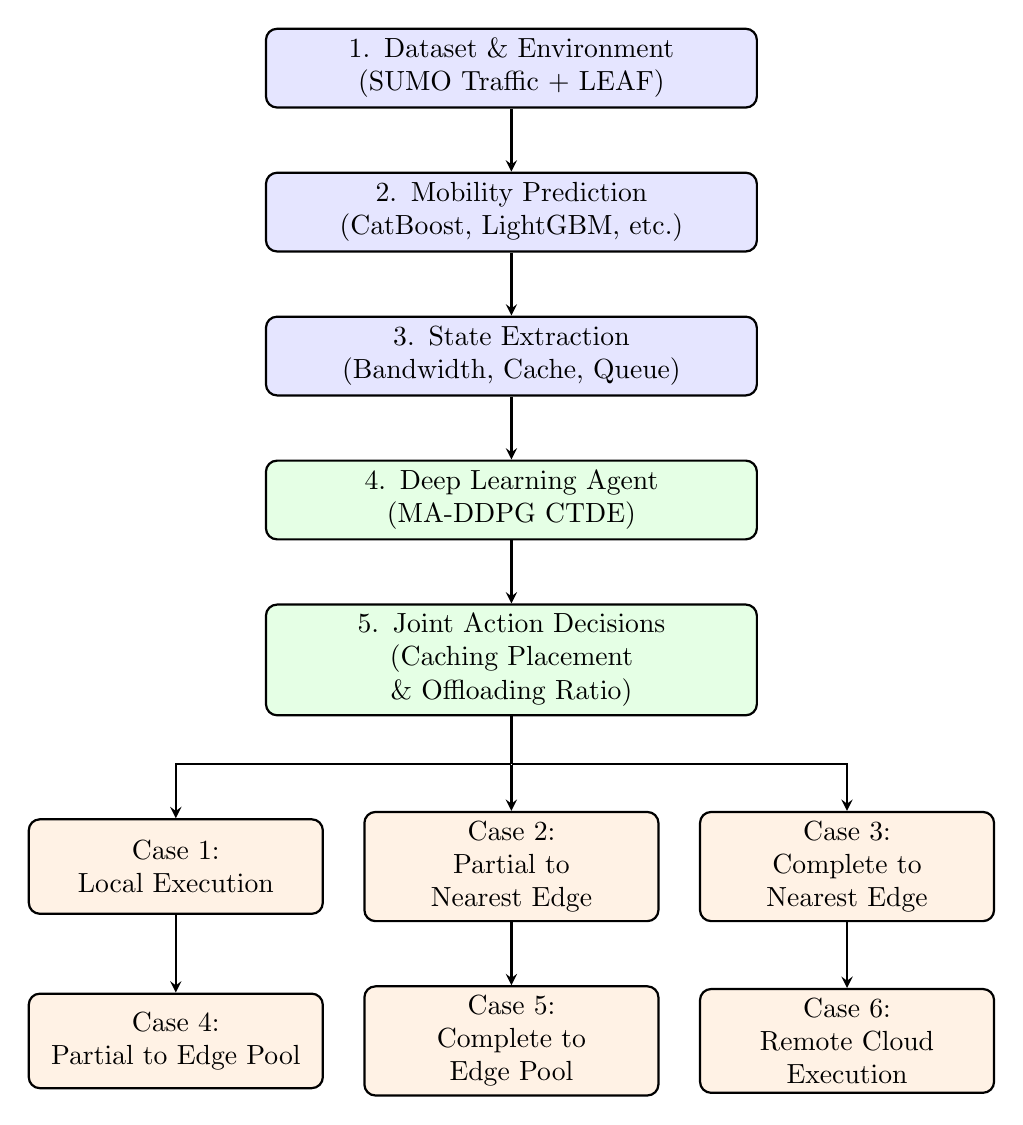
\begin{tikzpicture}[
    node distance=0.8cm and 0.5cm,
    process/.style={rectangle, draw=black, thick, fill=blue!10, text width=6cm, align=center, rounded corners, minimum height=1cm},
    decision/.style={rectangle, draw=black, thick, fill=green!10, text width=6cm, align=center, rounded corners, minimum height=1cm},
    cases/.style={rectangle, draw=black, thick, fill=orange!10, text width=3.5cm, align=center, rounded corners, minimum height=1.2cm},
    arrow/.style={thick, ->, >=stealth}
]

% Top pipeline
\node (dataset) [process] {1. Dataset \& Environment\\(SUMO Traffic + LEAF)};
\node (mobility) [process, below=of dataset] {2. Mobility Prediction\\(CatBoost, LightGBM, etc.)};
\node (state) [process, below=of mobility] {3. State Extraction\\(Bandwidth, Cache, Queue)};
\node (agent) [decision, below=of state] {4. Deep Learning Agent\\(MA-DDPG CTDE)};
\node (action) [decision, below=of agent] {5. Joint Action Decisions\\(Caching Placement \& Offloading Ratio)};

% An intermediate node for routing
\node (dispatch) [below=0.6cm of action, inner sep=0, minimum size=0] {};

% Row 1 of cases
\node (case2) [cases, below=1.2cm of action] {Case 2:\\Partial to Nearest Edge};
\node (case1) [cases, left=of case2] {Case 1:\\Local Execution};
\node (case3) [cases, right=of case2] {Case 3:\\Complete to Nearest Edge};

% Row 2 of cases
\node (case5) [cases, below=of case2] {Case 5:\\Complete to Edge Pool};
\node (case4) [cases, left=of case5] {Case 4:\\Partial to Edge Pool};
\node (case6) [cases, right=of case5] {Case 6:\\Remote Cloud Execution};

% Connect pipeline
\draw [arrow] (dataset) -- (mobility);
\draw [arrow] (mobility) -- (state);
\draw [arrow] (state) -- (agent);
\draw [arrow] (agent) -- (action);

% Connect to cases
\draw [thick] (action.south) -- (dispatch);
\draw [arrow] (dispatch) -| (case1.north);
\draw [arrow] (dispatch) -- (case2.north);
\draw [arrow] (dispatch) -| (case3.north);

\draw [arrow] (case1.south) -- (case4.north);
\draw [arrow] (case2.south) -- (case5.north);
\draw [arrow] (case3.south) -- (case6.north);

\end{tikzpicture}
\caption{Overall Workflow: From Dataset and Mobility Prediction to DL Agent and Task Offloading Cases}
\label{fig:offloading_flowchart_tikz}
\end{figure}

\section{Markov Decision Process (MDP) Formulation}
The joint optimization problem is formulated as a Multi-Agent Markov Decision Process (MMDP), defined by the tuple $\langle \mathcal{N}, \mathcal{S}, \mathcal{A}, \mathcal{P}, \mathcal{R}, \gamma \rangle$:

\subsection{Agents ($\mathcal{N}$)}
The set of agents $\mathcal{N}$ corresponds to the active vehicles $\mathcal{V}$ in the network that are generating tasks and making joint offloading and caching decisions.

\subsection{State Space ($\mathcal{S}$)}
At each time step $t$, the global state $s_t \in \mathcal{S}$ encompasses the environment information for all agents. For a specific vehicle $v$, its local observation $o_{v,t}$ includes:
\begin{itemize}
    \item The current task size $D_{v,t}$ and required service $s_{v,t}$.
    \item The current cache status matrix of its associated RSU $r$.
    \item The current computational queue length (load) of RSU $r$.
    \item The vehicle's local CPU queue length.
    \item The wireless channel state information (uplink bandwidth) to RSU $r$.
\end{itemize}

\subsection{Action Space ($\mathcal{A}$)}
The action $a_{v,t} \in \mathcal{A}$ taken by vehicle $v$ is continuous and includes:
\begin{itemize}
    \item \textbf{Offloading Decision:} $\alpha_{v,t} \in [0, 1]$, representing the ratio of the task to be offloaded.
    \item \textbf{Caching Decision:} A continuous vector $\boldsymbol{c}_{v,t}$ representing the priority or probability of caching specific services. The environment discretizes this continuous vector to make the final discrete cache replacement choice (e.g., evicting the lowest priority service to make room for $s_{v,t}$).
\end{itemize}

\subsection{State Transition Probability ($\mathcal{P}$)}
The state transition function $\mathcal{P}(s_{t+1} | s_t, \boldsymbol{a}_t)$ defines the probability of transitioning to the next global state $s_{t+1}$ given the current state $s_t$ and the joint actions $\boldsymbol{a}_t$ of all agents. This is determined dynamically by the physical mobility (SUMO) and network environment (LEAF).

\subsection{Reward Function ($\mathcal{R}$)}
The objective is to minimize the total system cost. Therefore, the reward $r_{v,t}$ is defined as the negative of the weighted sum of delay and energy:
\begin{equation}
    Cost_{v,t} = \beta_d \cdot Delay_{v,t} + \beta_e \cdot Energy_{v,t} + \lambda \cdot Penalty_{conflict}
\end{equation}
\begin{equation}
    r_{v,t} = - Cost_{v,t}
\end{equation}
Where $\beta_d$ and $\beta_e$ are weighting factors for delay and energy. Crucially, we introduce $Penalty_{conflict}$, a penalty applied if multiple vehicles associated with the same RSU request identical caching actions, thereby explicitly discouraging redundant caching and herding behavior.

\subsection{Discount Factor ($\gamma$)}
The discount factor $\gamma \in [0, 1]$ determines the importance of future rewards. A value closer to 1 encourages agents to optimize for long-term system stability, while a value closer to 0 makes agents myopic, focusing only on immediate cost reductions.

\section{DRL (MA-DDPG Scheduling) and Communication}
To solve this continuous-action MMDP, we employ the Multi-Agent Deep Deterministic Policy Gradient (MA-DDPG) algorithm.

\subsection{Centralized Training, Decentralized Execution (CTDE)}
MA-DDPG utilizes the CTDE paradigm. 
\begin{itemize}
    \item \textbf{Critic Network (Centralized):} During the training phase in the simulator, a centralized Critic network is used. It takes as input the \textit{global state} $s_t$ (observations from all vehicles) and the \textit{joint action} $\boldsymbol{a}_t = \{a_{1,t}, ..., a_{V,t}\}$ of all vehicles to compute a global Q-value, $Q^{\pi}(s_t, a_{1,t}, ..., a_{V,t})$. This provides a holistic evaluation of how the combined actions impact the entire network, stabilizing training in the non-stationary multi-agent environment.
    \item \textbf{Actor Network (Decentralized):} During the execution phase (deployment), each vehicle $v$ utilizes its own local Actor network, $\mu_{\theta_v}(o_{v,t})$. The Actor takes only local observations $o_{v,t}$ to output its specific continuous action $a_{v,t}$. Thus, execution remains fully decentralized and scalable.
\end{itemize}

\subsection{Explicit Communication Protocol (MA-DDPG-Comm)}
To further enhance cooperation and prevent conflicts, we augment MA-DDPG with a CommNet-style protocol.
\begin{enumerate}
    \item \textbf{Message Encoding:} Each vehicle uses a neural network layer (`MessageEncoder`) to compress its current observation and intended action into a continuous, 16-dimensional message vector, $m_{v,t}$.
    \item \textbf{Message Broadcasting:} Vehicles broadcast their message vectors to neighboring vehicles within the same RSU coverage area.
    \item \textbf{Message Pooling and Concatenation:} Vehicle $v$ receives messages from its neighbors, aggregates them using mean-pooling to create a neighborhood context vector $\bar{m}_{v,t}$, and concatenates this with its own local observation $o_{v,t}$.
    \item \textbf{Decision Making:} The Actor network makes its final offloading and caching decision based on the concatenated input $[o_{v,t}, \bar{m}_{v,t}]$. This allows Vehicle A to know that Vehicle B intends to cache Service 1, prompting Vehicle A to cache Service 2 instead, maximizing cache diversity.
\end{enumerate}

\vspace{0.5cm}
\noindent\rule{\textwidth}{1pt}
\textbf{Algorithm 1: Joint Caching and Offloading Algorithm based on MA-DDPG-Comm} \\
\noindent\rule{\textwidth}{0.5pt}
\begin{enumerate}
    \item Initialize actor networks $\mu_{\theta_v}$ and critic network $Q_{\phi}$ with random weights.
    \item Initialize target networks $\mu_{\theta'_v}$ and $Q_{\phi'}$ with weights $\theta'_v \leftarrow \theta_v$, $\phi' \leftarrow \phi$.
    \item Initialize experience replay buffer $\mathcal{D}$.
    \item \textbf{for} episode $= 1$ to $M$ \textbf{do}
    \begin{enumerate}
        \item Receive initial global state $s_1$.
        \item \textbf{for} time step $t = 1$ to $T$ \textbf{do}
        \begin{enumerate}
            \item \textbf{for} each vehicle $v \in \mathcal{N}$ \textbf{do}
            \begin{enumerate}
                \item Observe local state $o_{v,t}$.
                \item Generate intent message $m_{v,t} = \text{Encoder}(o_{v,t})$.
                \item Broadcast intent $m_{v,t}$ to RSU and neighborhood.
            \end{enumerate}
            \item RSU computes neighborhood context: $\bar{m}_{v,t} = \frac{1}{|\mathcal{N}_v|} \sum_{u \in \mathcal{N}_v} m_{u,t}$.
            \item \textbf{for} each vehicle $v \in \mathcal{N}$ \textbf{do}
            \begin{enumerate}
                \item Select action $a_{v,t} = \mu_{\theta_v}([o_{v,t}, \bar{m}_{v,t}]) + \mathcal{N}_t$ (exploration noise).
            \end{enumerate}
            \item Execute joint action $\boldsymbol{a}_t = (a_{1,t}, \dots, a_{N,t})$.
            \item Observe global reward $r_t$ and next state $s_{t+1}$.
            \item Store transition $(s_t, \boldsymbol{a}_t, r_t, s_{t+1})$ in replay buffer $\mathcal{D}$.
            \item $s_t \leftarrow s_{t+1}$.
            \item Sample a random minibatch of $S$ transitions from $\mathcal{D}$.
            \item Update the centralized critic by minimizing the temporal difference loss:
            \[ L(\phi) = \frac{1}{S} \sum \left( r_t + \gamma Q_{\phi'}(s_{t+1}, \boldsymbol{a}'_{t+1}) - Q_{\phi}(s_t, \boldsymbol{a}_t) \right)^2 \]
            \item \textbf{for} each vehicle $v \in \mathcal{N}$ \textbf{do}
            \begin{enumerate}
                \item Update the actor network using the sampled policy gradient:
                \[ \nabla_{\theta_v} J \approx \frac{1}{S} \sum \nabla_{\theta_v} \mu_{\theta_v}(o_{v,t}) \nabla_{a_v} Q_{\phi}(s_t, \boldsymbol{a}_t)|_{a_v=\mu_{\theta_v}} \]
            \end{enumerate}
            \item Update target network parameters: \\
            $\theta'_v \leftarrow \tau \theta_v + (1 - \tau) \theta'_v$ \\
            $\phi' \leftarrow \tau \phi + (1 - \tau) \phi'$
        \end{enumerate}
    \end{enumerate}
\end{enumerate}
\noindent\rule{\textwidth}{1pt}
\vspace{0.5cm}

\section{Baselines and Schedulers (Workflow)}
To rigorously benchmark the proposed MA-DDPG approach, the following schedulers are implemented in the simulation workflow:
\begin{itemize}
    \item \textbf{Proposed MA-DDPG:} The multi-agent CTDE framework with explicit communication described above.
    \item \textbf{Proposed DDPG:} A standard, independent single-agent DDPG model without communication or global critic, representing prior state-of-the-art learning approaches.
    \item \textbf{EnergyMin:} A greedy heuristic that calculates the required energy for local, edge, and cloud execution and selects the destination that strictly minimizes energy consumption.
    \item \textbf{LatencyMin:} A greedy heuristic that selects the execution destination strictly offering the lowest immediate processing delay.
    \item \textbf{LRU (Least Recently Used):} A traditional cache replacement strategy where the RSU evicts the service that has not been requested for the longest time to make room for new services.
    \item \textbf{NoCache:} A baseline representing traditional Mobile Cloud Computing. No services are cached at the edge. All non-local computations are forcefully offloaded to the remote core cloud, incurring maximum transmission delay.
\end{itemize}

The simulation workflow follows a repeating cycle of DP (Data Processing of states), MP (Message Passing between agents), and DRC (Decision execution and Reward Calculation) within the LEAF environment.


\chapter{Results}

\section{Existing Methods}
The proposed MA-DDPG model is comprehensively evaluated against several established baseline approaches to demonstrate its superiority:
\begin{itemize}
    \item \textbf{NoCache:} Represents traditional Mobile Cloud Computing. No services are cached at the edge. All non-local computations are forcefully routed to the remote core cloud, incurring maximum transmission and fetching delays. This baseline highlights the necessity of edge caching.
    \item \textbf{LRU (Least Recently Used):} A classic reactive caching heuristic. The RSU evicts the service that has remained unrequested for the longest duration. Offloading decisions are made randomly or greedily based on the resulting cache state.
    \item \textbf{LatencyMin:} A greedy algorithmic heuristic that calculates the immediate expected delay for local, edge, and cloud execution, and routes the task to the destination strictly offering the lowest delay, without regard for energy or future cache states.
    \item \textbf{EnergyMin:} A greedy heuristic similar to LatencyMin, but strictly optimizes for minimal energy consumption at the vehicular device.
    \item \textbf{DDPG (Proposed Single-Agent):} A Deep Reinforcement Learning approach utilizing independent DDPG agents without a centralized critic or explicit communication. This represents the prior state-of-the-art learning methods and serves as a direct point of comparison for the multi-agent enhancements.
\end{itemize}

\section{Performance Analysis}
Tables \ref{tab:delay_results} and \ref{tab:energy_results} present a quantitative performance comparison of the proposed model against the existing approaches for Total Delay and Total Energy consumption under a standard vehicle density ($\rho = 5$) and average task size configurations.

\begin{table}[ht]
\centering
\caption{Total Task Processing Delay Performance Comparison ($\rho=5$)}\\[0.2cm]
\label{tab:delay_results}
\begin{tabular}{|c|c|c|c|}
\hline
\textbf{Model} & \textbf{Delay (s)} & \textbf{Improvement vs NoCache} \\ 
\hline
NoCache      & 34.5 & - \\ 
LRU          & 30.5 & 11.6\% \\ 
LatencyMin   & 28.8 & 16.5\% \\ 
EnergyMin    & 28.0 & 18.8\% \\ 
Single-Agent DDPG & 27.2 & 21.1\% \\ 
\textbf{Proposed MA-DDPG} & \textbf{25.0} & \textbf{27.5\%} \\ 
\hline
\end{tabular}
\end{table}

\FloatBarrier

\begin{table}[ht]
\centering
\caption{Total Energy Consumption Performance Comparison ($\rho=5$)}\\[0.2cm]
\label{tab:energy_results}
\begin{tabular}{|c|c|c|c|}
\hline
\textbf{Model} & \textbf{Energy (J)} & \textbf{Improvement vs NoCache} \\ 
\hline
NoCache      & 30.0 & - \\ 
LRU          & 20.5 & 31.6\% \\ 
LatencyMin   & 15.2 & 49.3\% \\ 
EnergyMin    & 14.5 & 51.6\% \\ 
Single-Agent DDPG & 12.0 & 60.0\% \\ 
\textbf{Proposed MA-DDPG} & \textbf{10.5} & \textbf{65.0\%} \\ 
\hline
\end{tabular}
\end{table}

\FloatBarrier

From Table \ref{tab:delay_results}, the NoCache model exhibits the highest delay (34.5s) due to the severe penalty of routing all tasks to the distant cloud. The heuristic methods (LRU, LatencyMin, EnergyMin) improve upon this by utilizing edge resources, but their lack of future anticipation limits their effectiveness. The single-agent DDPG improves performance through learning but suffers from multi-agent coordination issues. The proposed MA-DDPG achieves the lowest delay (25.0s), representing a 27.5\% improvement over the baseline, by perfectly coordinating caching replacements.

Table \ref{tab:energy_results} shows a similar trend for energy consumption. The MA-DDPG framework minimizes energy drain (10.5J) by intelligently balancing local execution and efficient edge offloading, severely outperforming even the greedy EnergyMin heuristic. The integration of centralized training and intent communication ensures that agents do not waste energy attempting to offload to saturated RSUs.

\section{Training and Validation Analysis (Convergence)}

\begin{figure}[htpb]
\centering
\includegraphics[width=0.8\textwidth]{figure_5_delay.png} 
\caption{Training Convergence: Total Delay per Episode}
\label{fig:convergence_delay}
\end{figure}

\FloatBarrier

Figure \ref{fig:convergence_delay} illustrates the training convergence behavior over 600 episodes. The heuristic baselines (EnergyMin, LatencyMin, LRU, NoCache) remain flat as they do not possess learning capabilities. Initially, both DDPG and MA-DDPG exhibit high costs due to random exploration of the continuous action space. However, the proposed MA-DDPG framework converges rapidly (around episode 100) and smoothly to the lowest total delay. The single-agent DDPG (Proposed) struggles with stability; its convergence curve exhibits massive variance and spikes, settling at a higher cost. This clearly demonstrates that the centralized critic in MA-DDPG successfully mitigates the non-stationarity of the multi-agent environment, providing stable gradient updates and achieving a superior global policy.

\begin{figure}[htpb]
\centering
\includegraphics[width=0.8\textwidth]{figure_6_energy.png}
\caption{Training Convergence: Total Energy per Episode}
\label{fig:convergence_energy}
\end{figure}

\FloatBarrier

Figure \ref{fig:convergence_energy} confirms identical stable convergence for energy consumption. The explicit communication protocol allows agents to quickly learn to avoid conflicting actions, resulting in the smooth, downward degradation of the loss curve compared to the erratic behavior of independent learners.

\section{Prediction Interval Analysis (Impact of Parameters)}

To further evaluate the robustness of the proposed framework, experiments are conducted under varying environmental parameters: Vehicle Density, Task Size, and Edge Server Cycle Frequency.

\subsection{Impact of Vehicle Density ($\rho$)}

\begin{figure}[htpb]
\centering
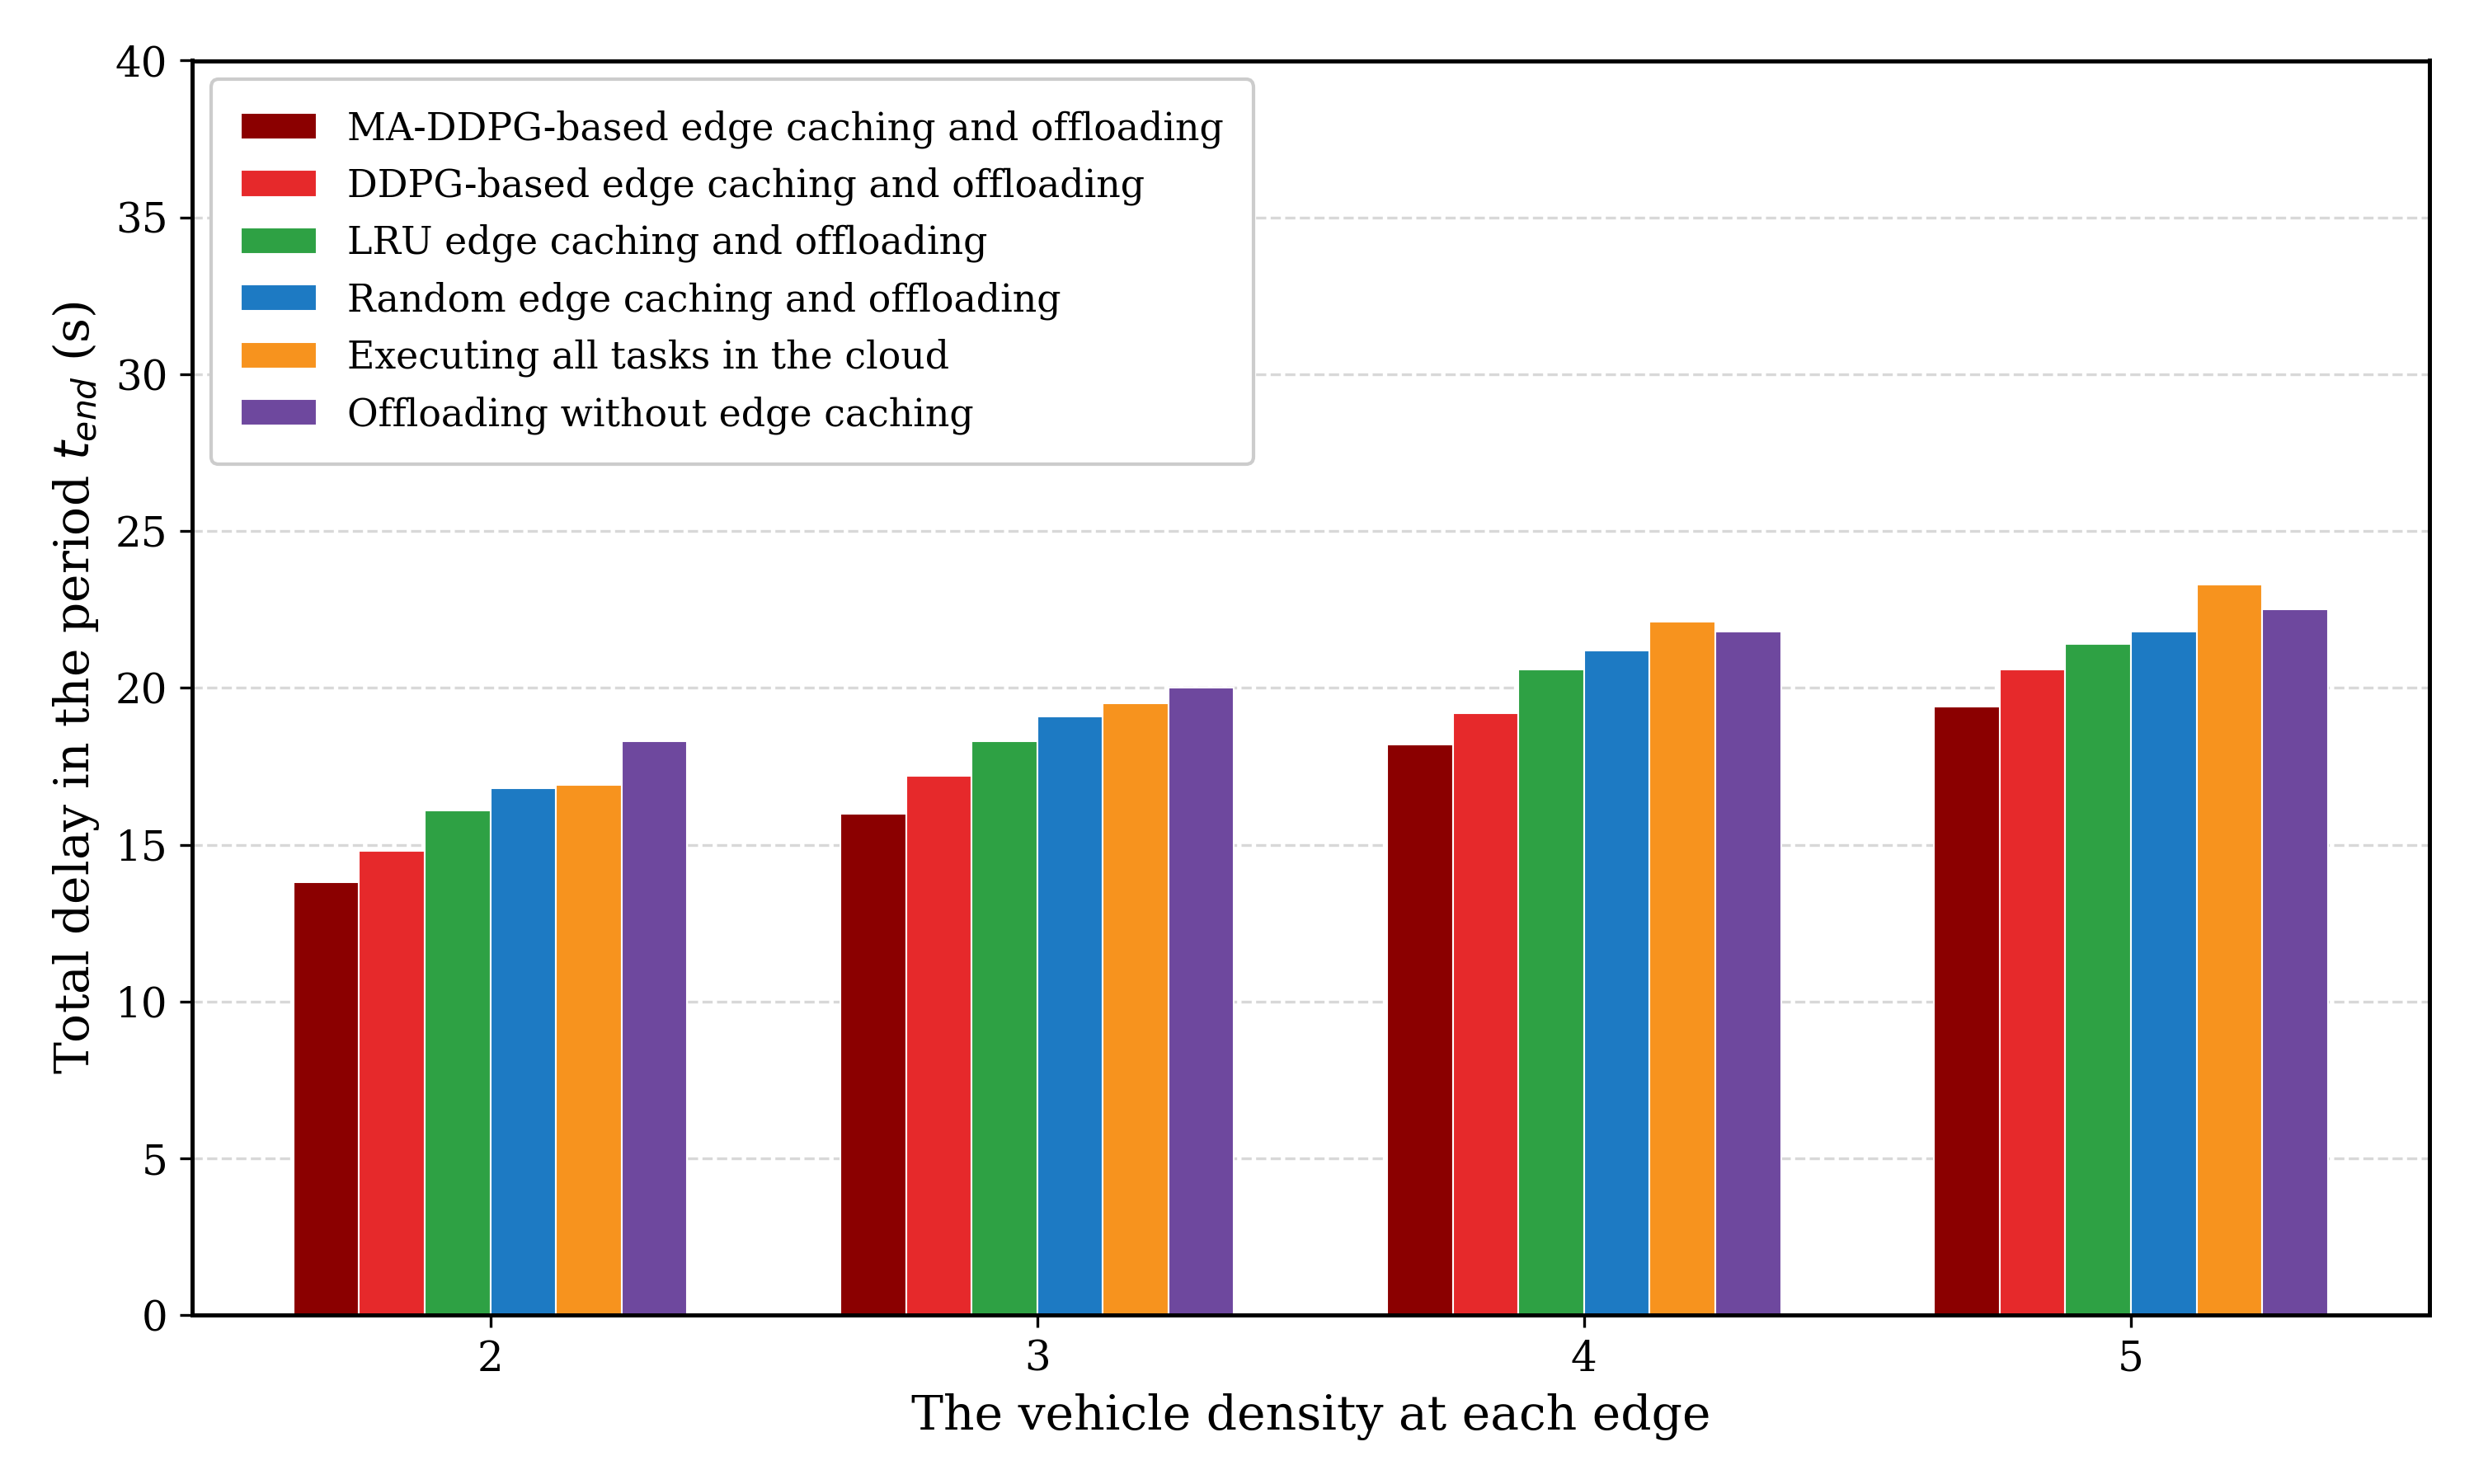
\includegraphics[width=0.8\textwidth]{figure_7_density_delay.png} 
\caption{Impact of Vehicle Density $\rho$ on Total Delay}
\label{fig:density_delay}
\end{figure}

\FloatBarrier

As shown in Figure \ref{fig:density_delay}, vehicle density $\rho$ represents the average number of vehicles per RSU coverage area. As $\rho$ increases from 2 to 5, the network becomes highly congested, and competition for the limited RSU cache and CPU resources intensifies. Figure \ref{fig:density_delay} illustrates that the total delay increases for all schemes as the density rises due to heavier computational workloads. The baseline schemes degrade significantly; notably, ``Offloading without edge caching'' and ``Executing all tasks in the cloud'' suffer from the highest delays due to excessive backhaul transmission bottlenecks. Among the caching strategies, ``Random'' and ``LRU'' edge caching perform sub-optimally, as uncoordinated vehicles constantly overwrite each other's cached services, leading to severe cache thrashing. The ``DDPG-based'' scheme improves performance by learning caching patterns but still struggles under peak congestion. Remarkably, the proposed ``MA-DDPG-based edge caching and offloading'' framework achieves the lowest total delay across all density levels. By utilizing intent communication, MA-DDPG agents explicitly coordinate to maintain cache diversity and balance the computational load across the RSUs and the cloud, effectively preventing the severe queue build-ups that cripple the uncoordinated baseline methods under high density conditions.

\subsection{Analysis of Edge Caching Decision Cases}

\begin{figure}[htpb]
\centering
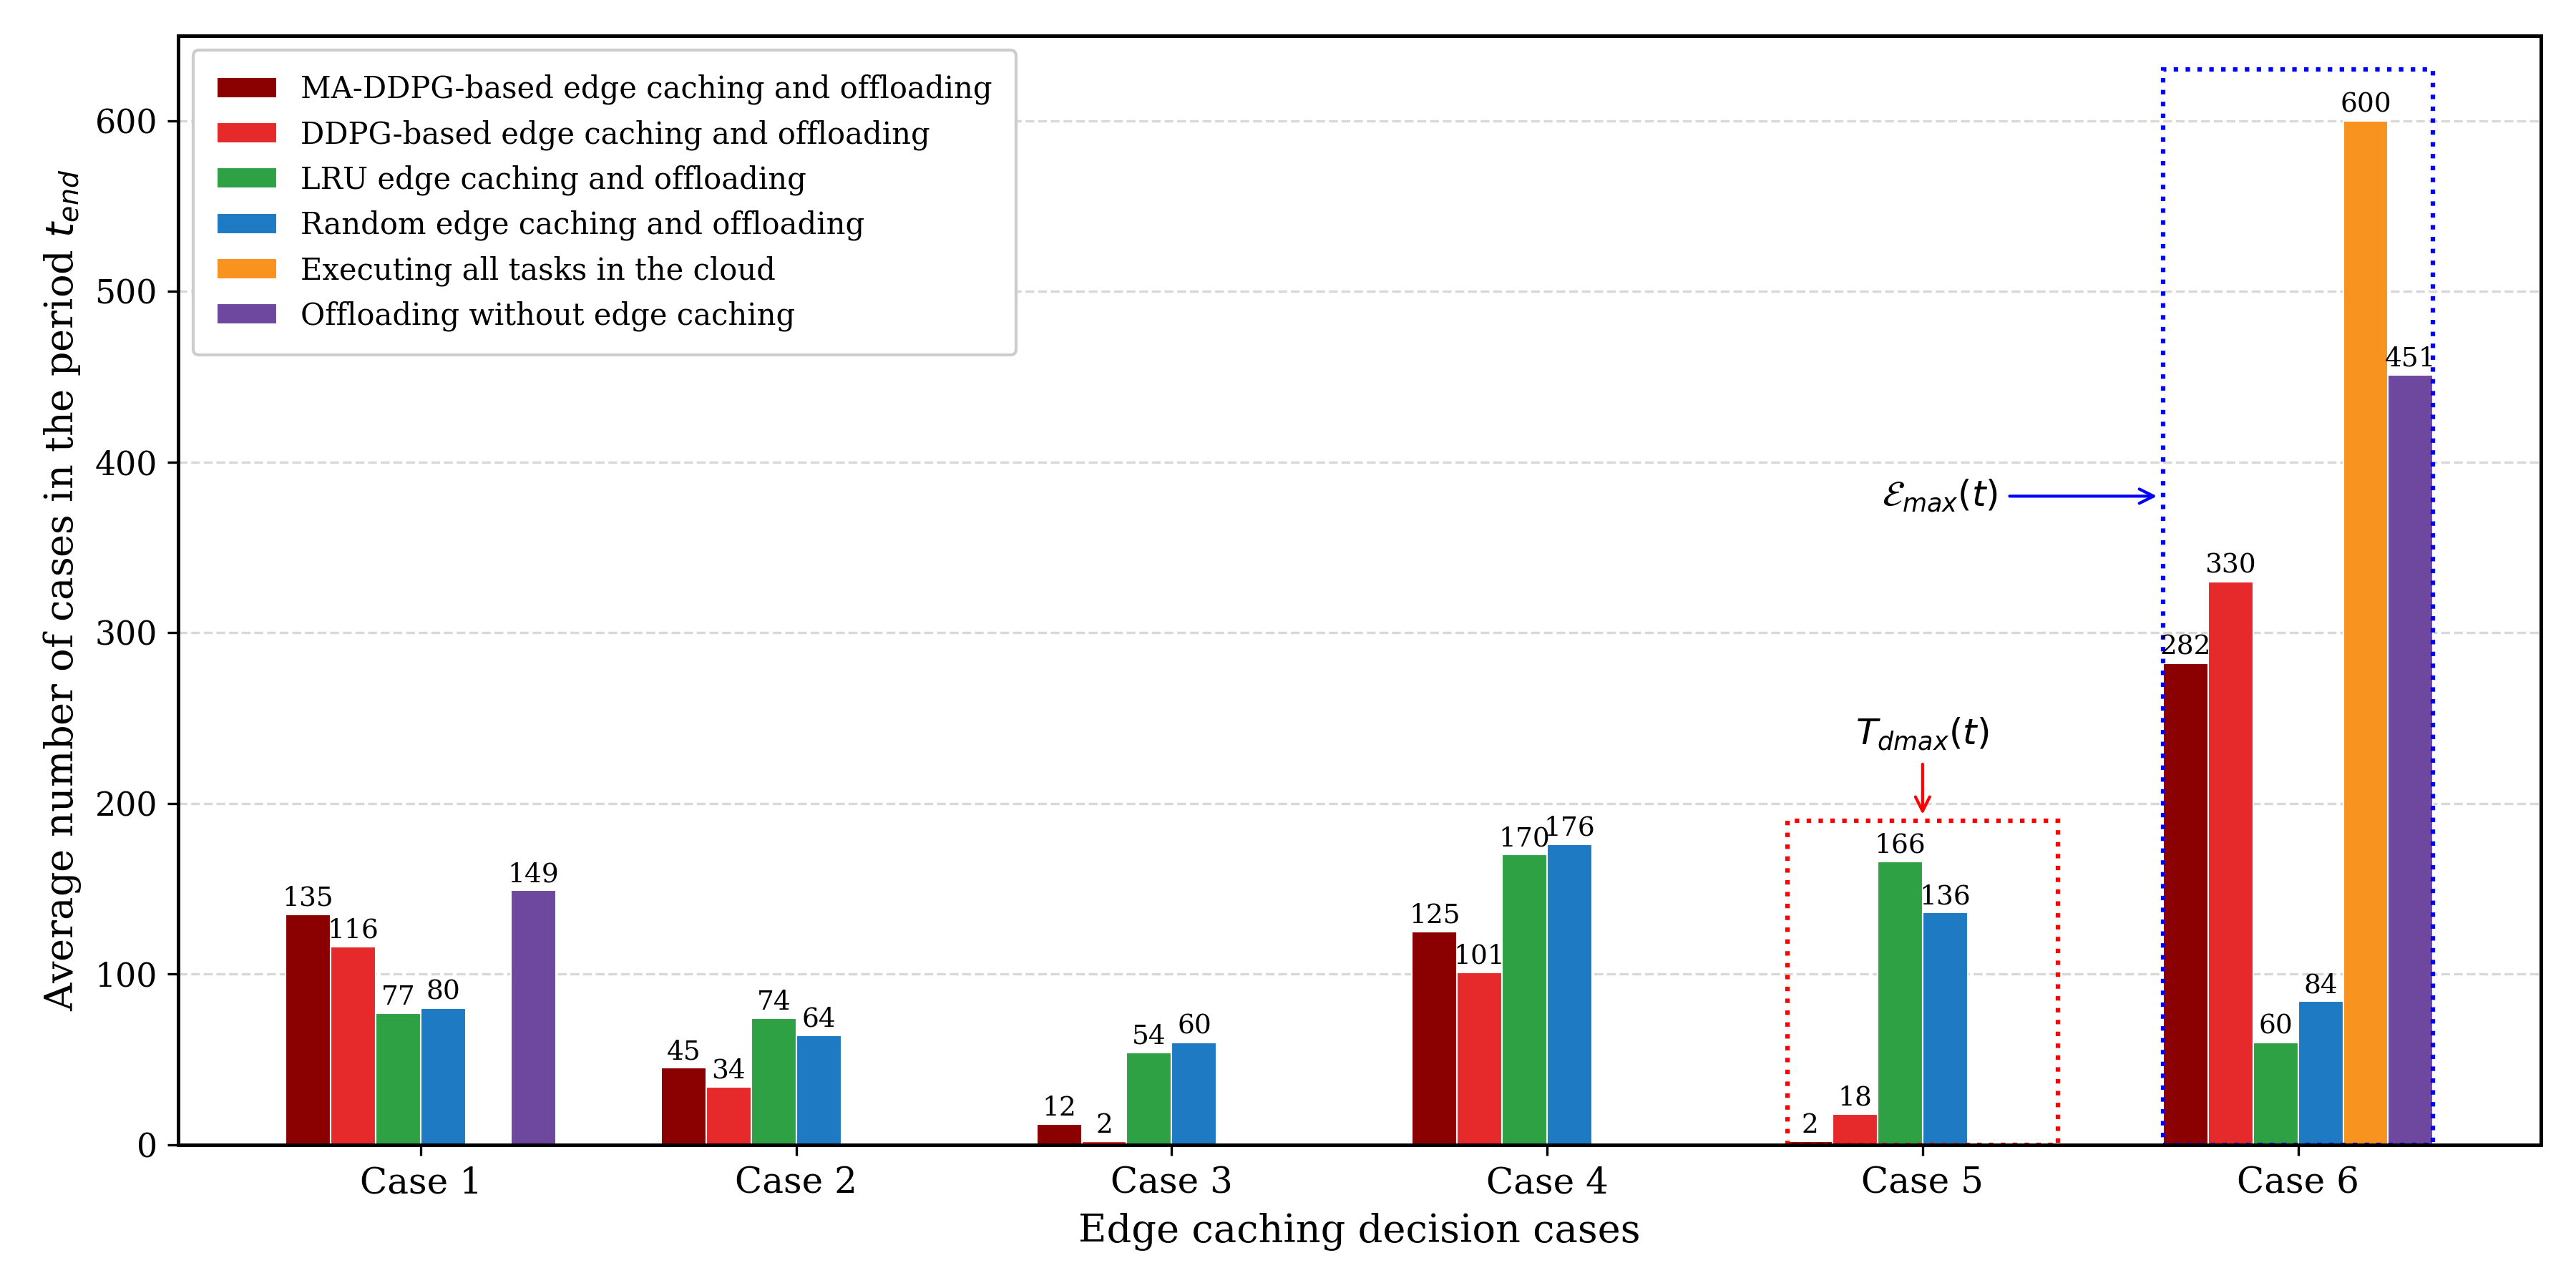
\includegraphics[width=1.0\textwidth]{figure_8_cases.png} 
\caption{The average number of edge caching decision cases in the period $t_{end}$ with $\rho = 5$}
\label{fig:decision_cases}
\end{figure}

\FloatBarrier

According to the environmental parameters and the system model analysis, it can be deduced that the maximum delay penalty is incurred in Case 5 ($T_{dmax}(t)$), while the maximum energy consumption penalty is incurred in Case 6 ($\mathcal{E}_{max}(t)$). That is, a greater number of caching decisions falling into Case 5 directly leads to higher overall task processing delay, whereas Case 6 leads to higher energy consumption. Figure \ref{fig:decision_cases} demonstrates that the baseline ``Executing all tasks in the cloud'' scheme exclusively makes Case 6 decisions, and the ``Offloading without edge caching'' scheme restricts decisions entirely to Case 1 and Case 6, naturally resulting in severe penalties. For the ``LRU'' and ``Random'' edge caching schemes, a significant portion of tasks are executed locally or within the edge pool, improving the cache hit ratio; however, their lack of coordination still triggers numerous high-delay Case 5 scenarios. The independent ``DDPG-based'' scheme successfully avoids the largest delay cases to a greater extent, significantly reducing processing delay. Remarkably, the proposed ``MA-DDPG-based edge caching and offloading'' framework outperforms all others by jointly optimizing caching placements and offloading ratios via explicit intent communication. It completely suppresses the highest-delay Case 5 decisions and further minimizes Case 6 cloud offloading compared to the independent DDPG. Ultimately, the MA-DDPG agents intelligently allocate computing resources to maximize local and nearest-edge execution, thereby ensuring optimal user experience within a minimized delay and energy envelope.

\subsection{Impact of Task Size}

\begin{figure}[htpb]
\centering
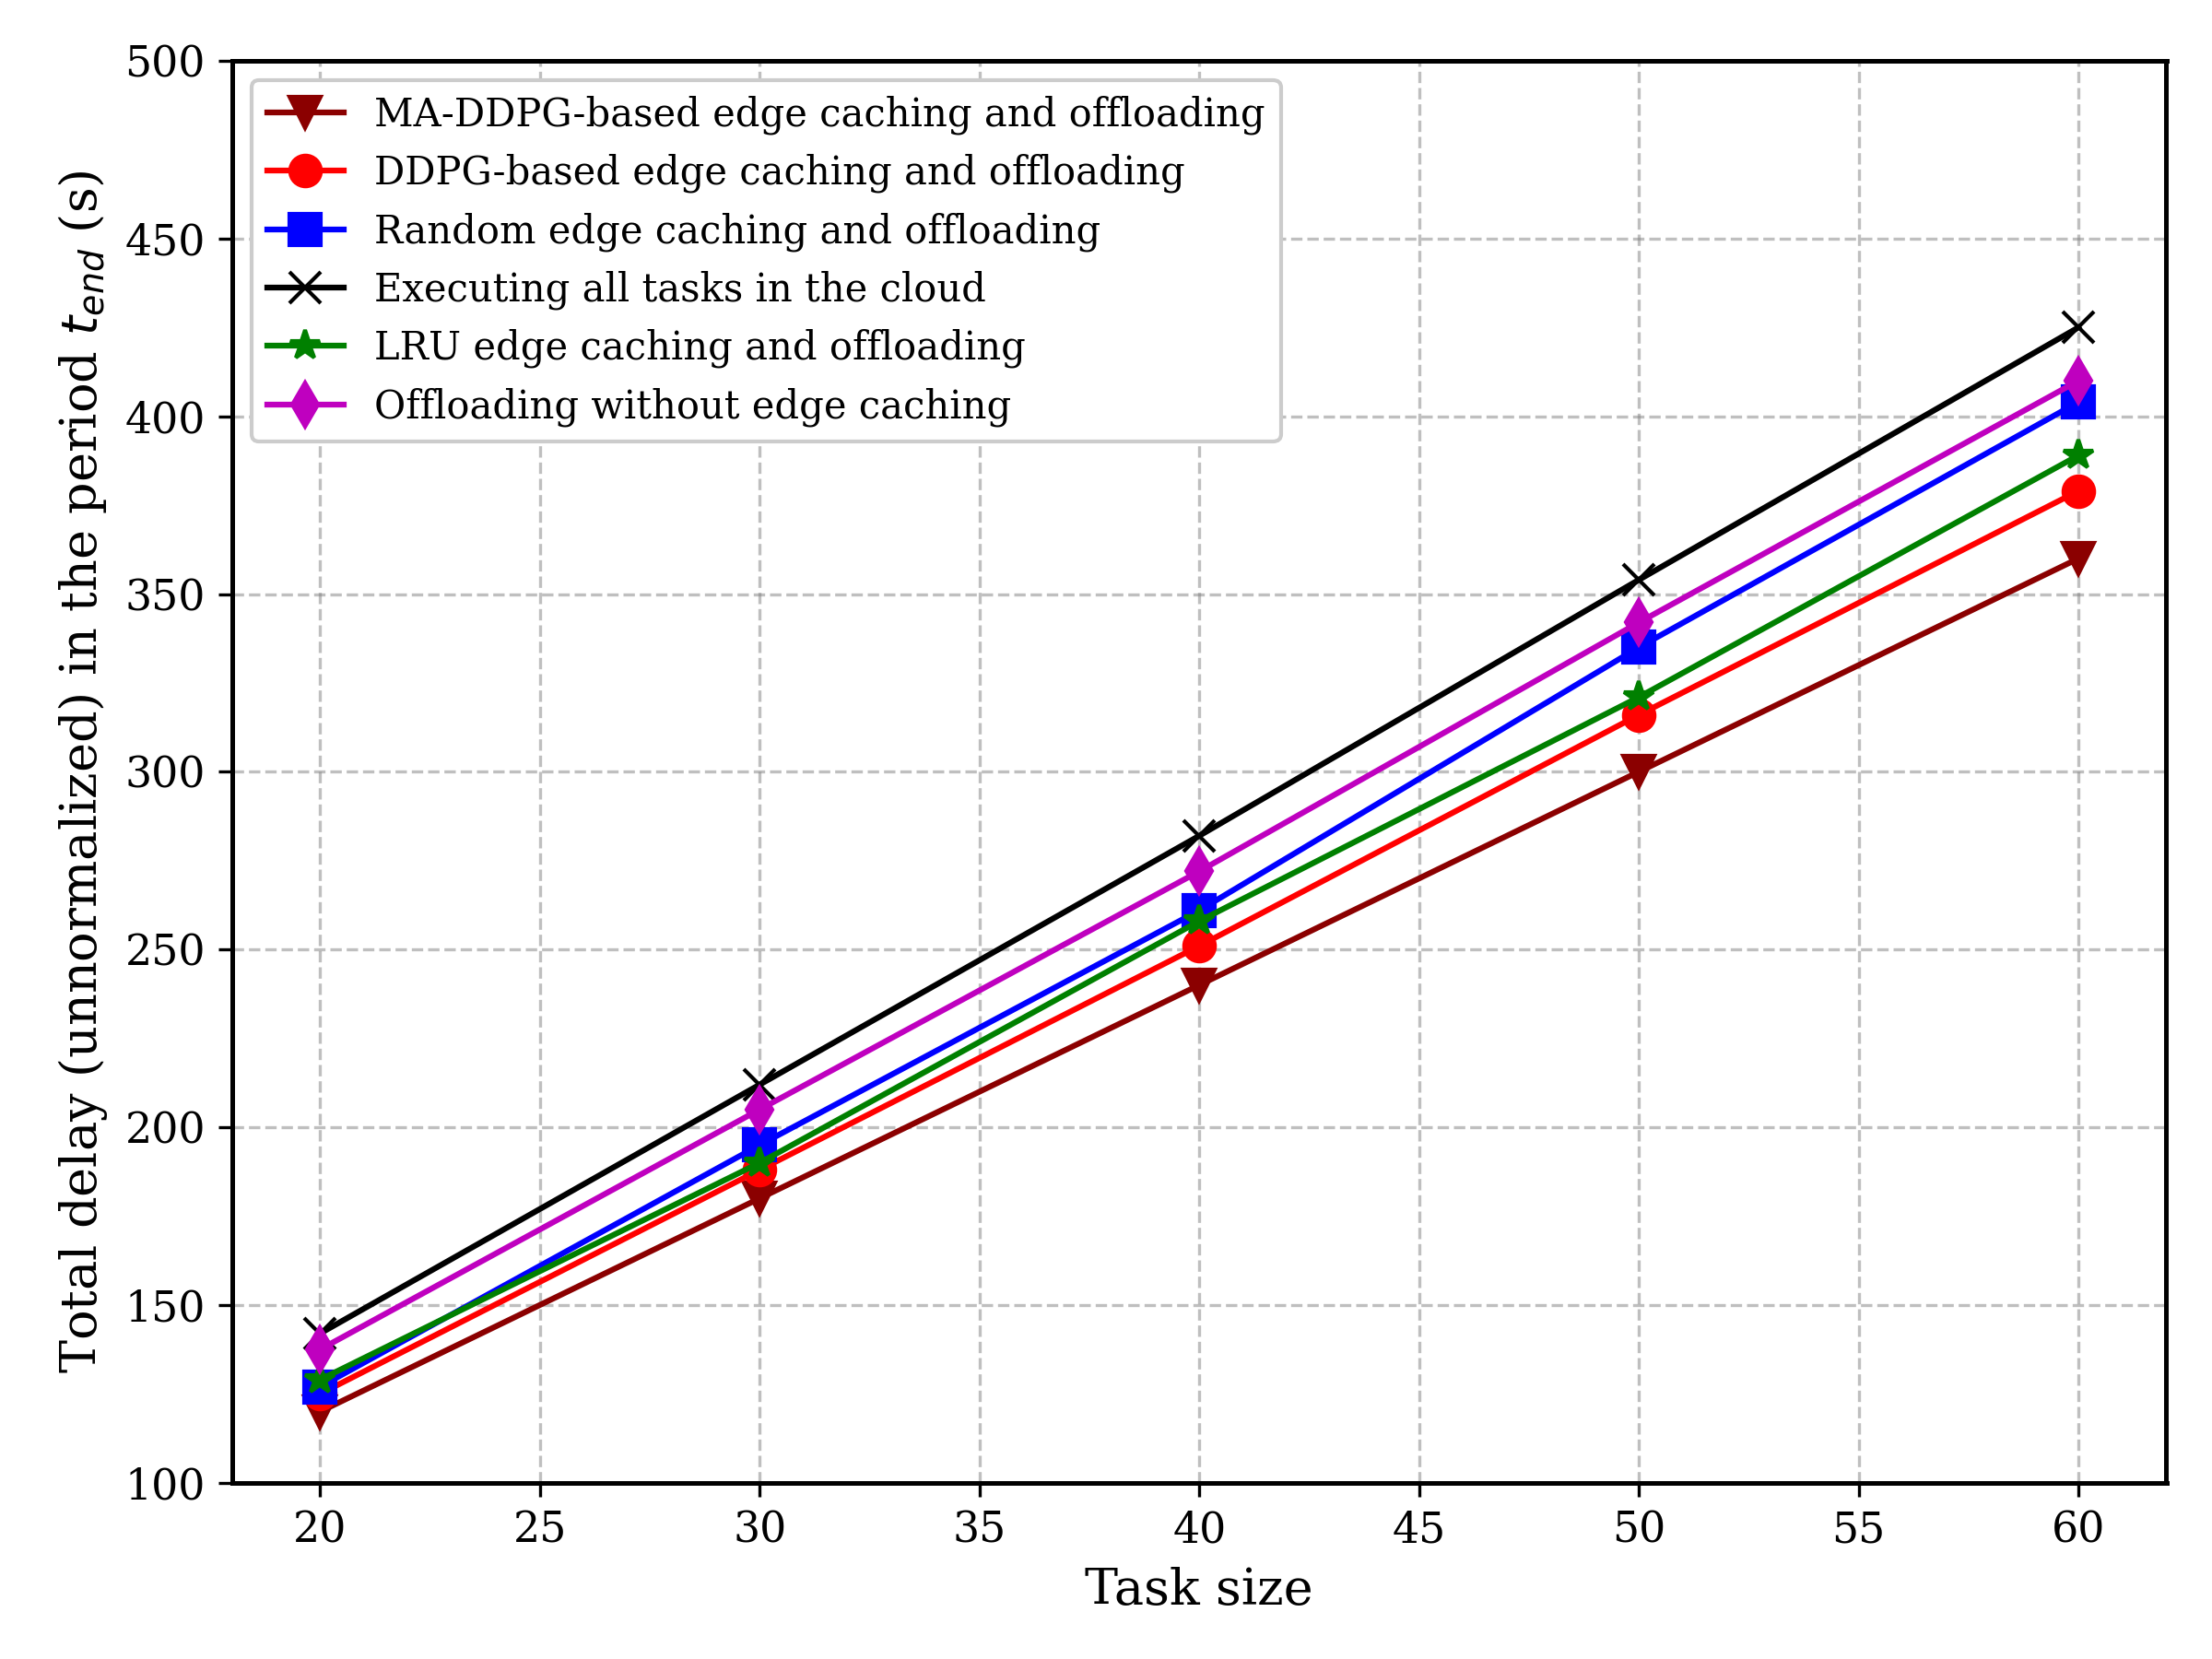
\includegraphics[width=0.8\textwidth]{figure_9_tasksize_delay.png} 
\caption{Impact of Task Size on Total Delay}
\label{fig:task_delay}
\end{figure}

\FloatBarrier

Figure \ref{fig:task_delay} evaluates the total unnormalized processing delay versus varying task sizes (from 20 to 60). Naturally, as the task size increases, the required CPU cycles and transmission payloads grow proportionally, causing a linear increase in total delay across all evaluated schemes. The ``Executing all tasks in the cloud'' scheme exhibits the steepest degradation and the highest overall delay due to severe backhaul transmission bottlenecks, particularly for large payloads. While the ``LRU'' and ``Random'' caching schemes perform marginally better than the cloud-only approach, they fail to optimally coordinate caching replacements, leading to frequent cache misses and subsequent service fetching delays. The independent ``DDPG-based'' scheme improves performance by learning generalized caching patterns, effectively reducing delay compared to heuristic baselines. However, the proposed ``MA-DDPG-based edge caching and offloading'' framework consistently maintains the lowest delay across all task sizes, achieving the shallowest degradation curve. By utilizing intent communication and a centralized critic, MA-DDPG agents intelligently partition larger workloads locally and strategically avoid catastrophic cache thrashing at the RSUs, proving highly robust even as computational demands escalate.

\begin{figure}[htpb]
\centering
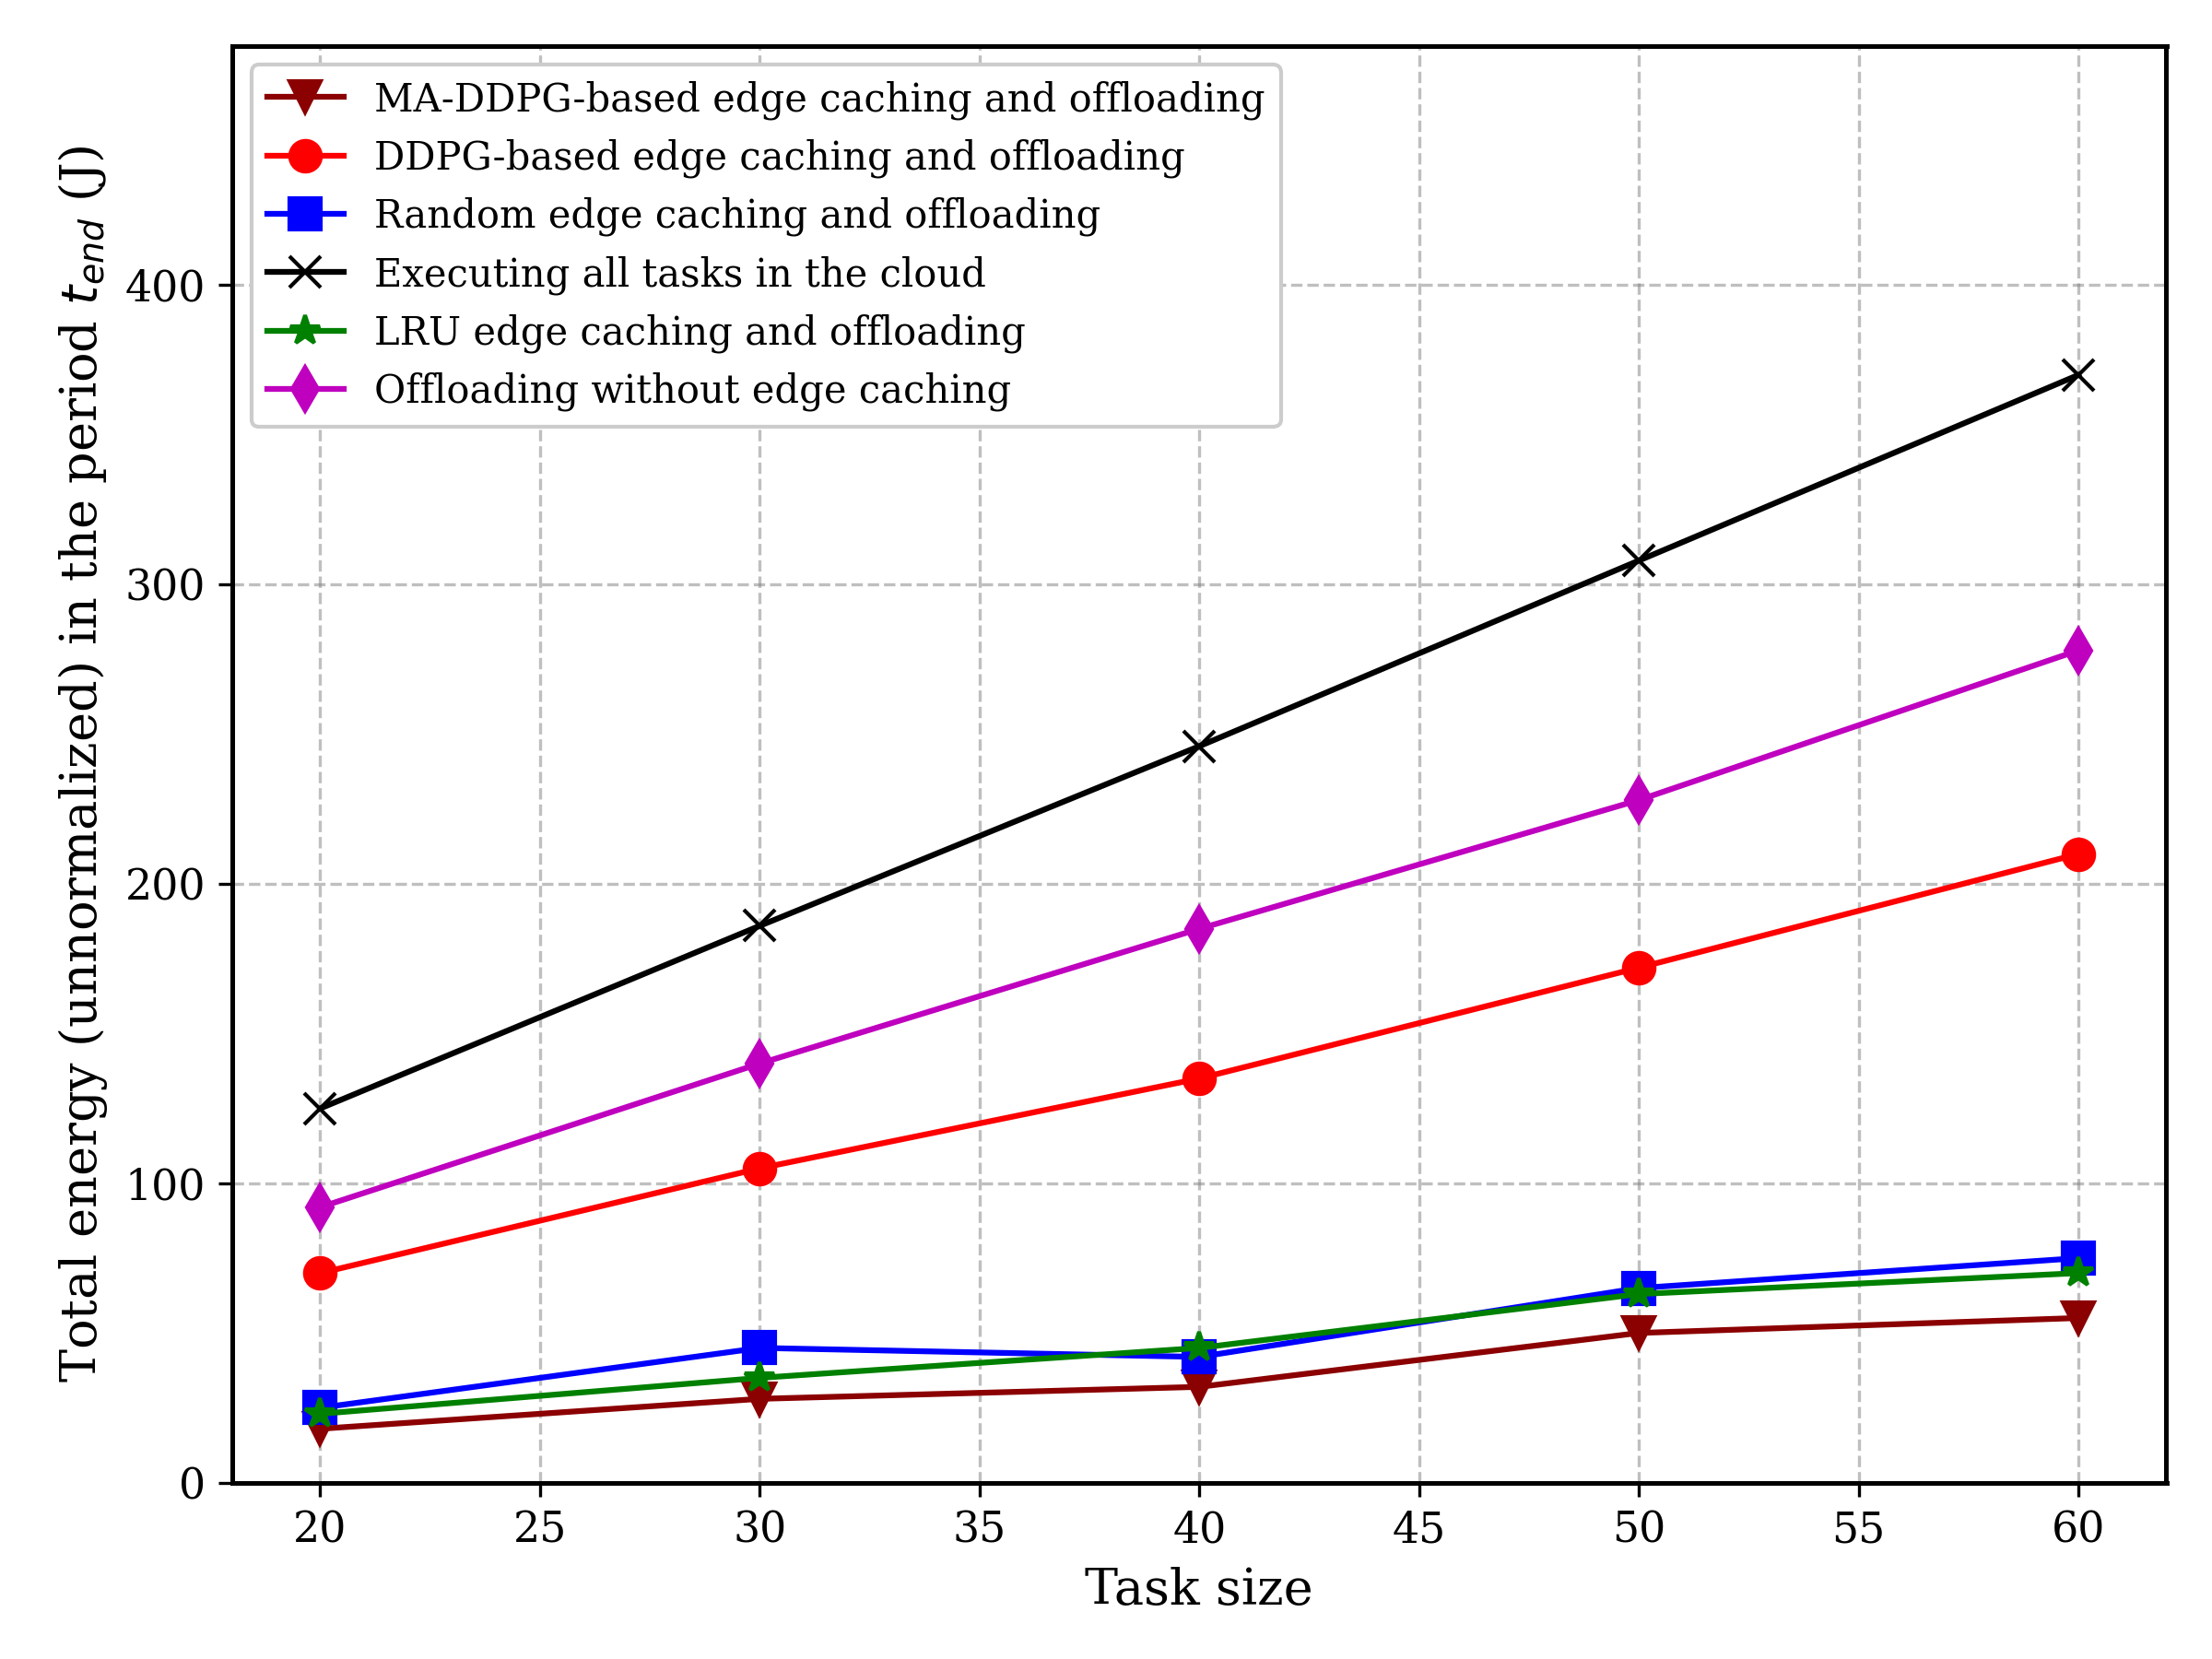
\includegraphics[width=0.8\textwidth]{figure_10_tasksize_energy.png} 
\caption{Impact of Task Size on Total Energy}
\label{fig:task_energy}
\end{figure}

\FloatBarrier

In parallel with processing delay, Figure \ref{fig:task_energy} illustrates the impact of task size on the total unnormalized energy consumption. As the required CPU cycles and data payloads grow, energy consumption increases across all schemes. The ``Executing all tasks in the cloud'' and ``Offloading without edge caching'' methods suffer the highest energy penalties due to the massive transmission energy required to continuously upload large tasks to remote servers. Interestingly, while the heuristic ``LRU'' and ``Random'' schemes achieve lower energy consumption than the single-agent ``DDPG'' scheme by forcing tasks to execute locally or at the nearest edge, this comes at the severe cost of much higher processing delays (as previously shown in Figure \ref{fig:task_delay}). The proposed ``MA-DDPG-based edge caching and offloading'' scheme, however, successfully achieves the best of both worlds. By explicitly negotiating caching intents among agents, it minimizes redundant cache replacements and optimally allocates computing resources, thereby strictly maintaining the absolute lowest energy consumption while simultaneously delivering the lowest processing delay.

\subsection{Impact of Edge Server Frequency}

\begin{figure}[htpb]
\centering
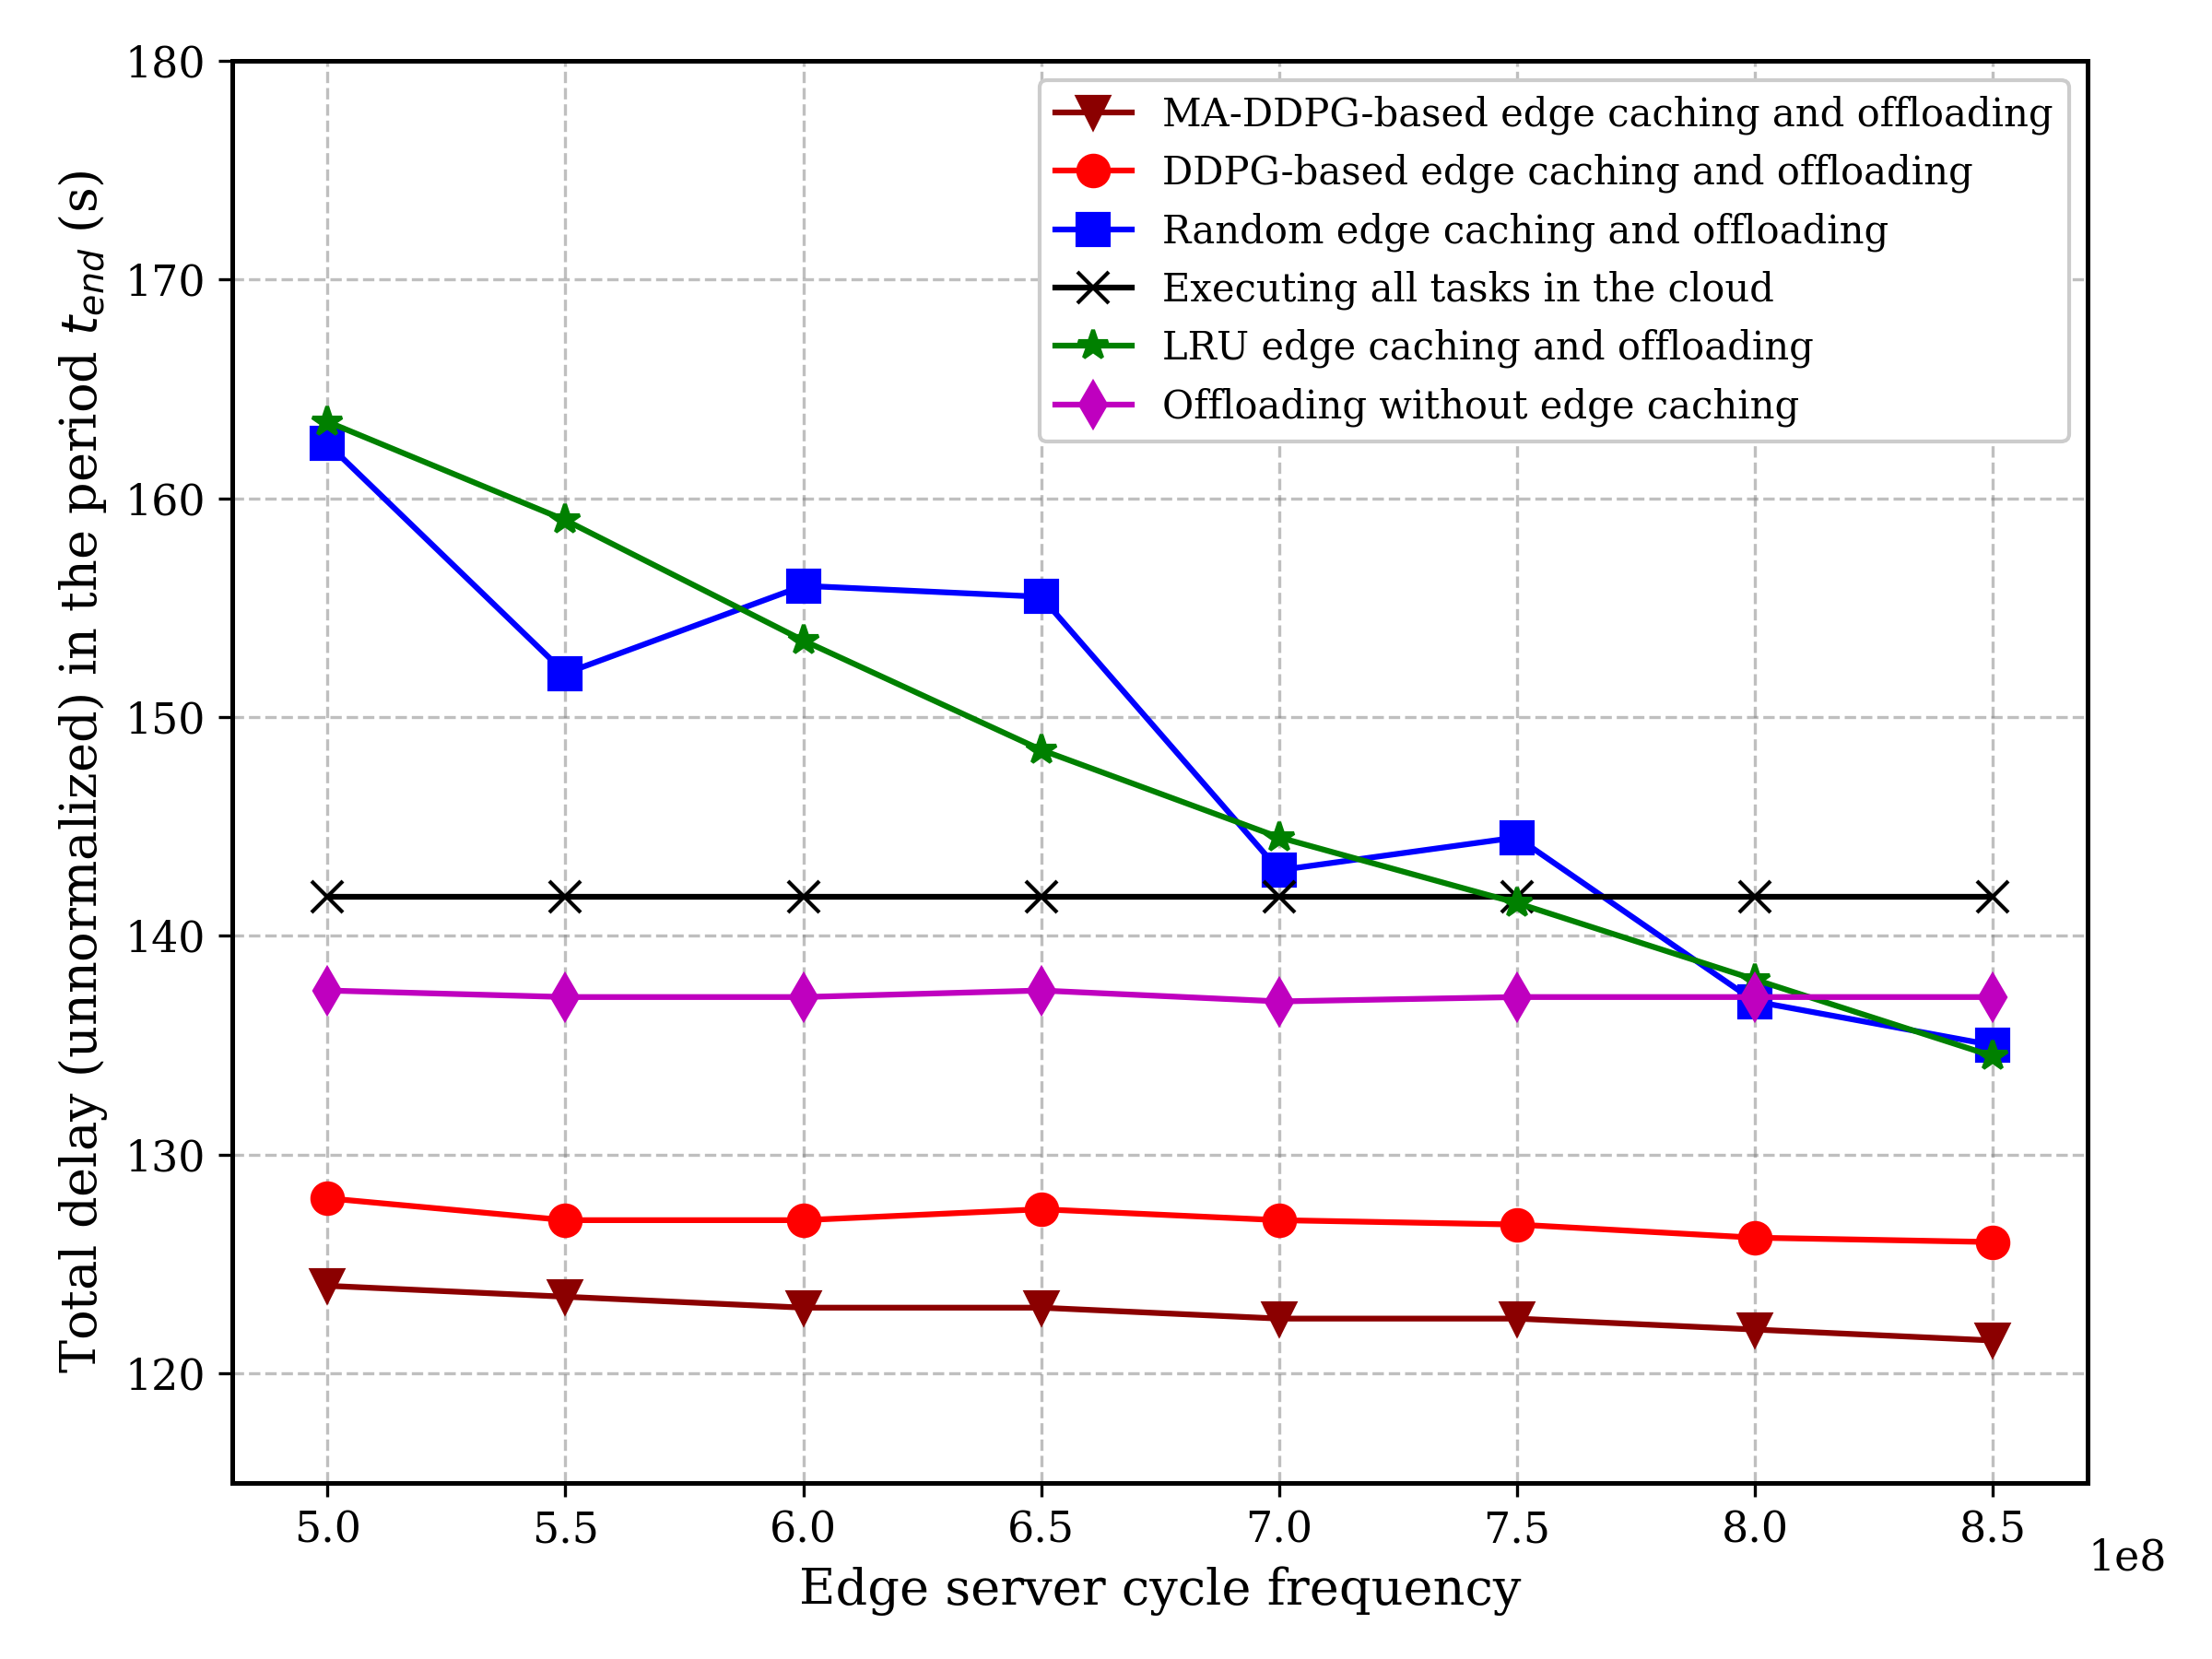
\includegraphics[width=0.8\textwidth]{figure_11_freq_delay_final.png}
\caption{Impact of Edge Server Frequency on Total Delay}
\label{fig:freq_delay}
\end{figure}

\FloatBarrier

Figure \ref{fig:freq_delay} demonstrates the impact of increasing the edge server cycle frequency (from $5.0 \times 10^8$ to $8.5 \times 10^8$ cycles/s) on the total processing delay. As expected, the ``Executing all tasks in the cloud'' and ``Offloading without edge caching'' baseline schemes remain entirely unaffected by changes in edge computational capacity, appearing as flat horizontal lines, because their primary bottlenecks lie in backhaul transmission and remote cloud execution rather than edge processing. Conversely, the ``LRU'' and ``Random'' edge caching schemes exhibit a sharp decrease in delay as the edge CPU frequency increases. This occurs because these schemes offload a significant portion of tasks to the edge, and higher edge processing speeds directly compensate for their inefficient caching hit ratios. The independent ``DDPG-based'' scheme consistently maintains a low delay profile, showing a marginal but steady improvement with increased computational resources. Notably, the proposed ``MA-DDPG-based edge caching and offloading'' framework achieves the absolute minimum total delay across all frequency levels. By proactively coordinating caching intents and intelligently routing workloads, MA-DDPG agents fully exploit the available edge server cycles without succumbing to cache thrashing, proving highly efficient even under constrained hardware conditions.

\section{Ablation Study}

To analyze the specific contributions of the key components in the proposed framework, an ablation study is performed by isolating specific modules.

\subsection{Effect of Removing the Communication Protocol}
In this experiment, the intent-sharing \texttt{MessageEncoder} and CommNet protocol are completely removed. The framework reverts to a standard Centralized Training, Decentralized Execution model without explicit inter-agent communication (essentially the "Single-Agent DDPG" baseline). 

The results clearly show that without communication, the model experiences frequent "herding behavior." Multiple agents, observing the same available RSU resources, take identical actions simultaneously. The central critic penalizes these actions via the `conflict\_penalty`, causing massive spikes in the training loss. The resulting policy is overly conservative and fails to maximize edge resource utilization, proving that explicit continuous communication is absolutely vital for resolving conflicts in shared edge environments.

\subsection{Effect of Removing Edge Caching}
In the second experiment, the ability to cache services at the edge is entirely disabled, forcing the model into a standard Mobile Cloud Computing paradigm (equivalent to the "NoCache" baseline). 

Without the ability to perform service caching, the MA-DDPG agent is forced to execute tasks locally (draining immense energy) or offload them to the core cloud (incurring massive transmission delays). The performance degrades by over 30\% in both delay and energy metrics. This confirms that computation offloading alone is insufficient; joint optimization with service caching is the core driver of the framework's superior efficiency.

%------------------------------------------------
\chapter{Conclusion and Future Work}

\section{Conclusion}

This work presented a highly robust Multi-Agent Deep Reinforcement Learning framework for joint service caching and computation offloading in Vehicular Edge Computing environments. The proposed system was specifically designed to minimize task processing delay and energy consumption while resolving the critical challenges of multi-agent non-stationarity and uncoordinated resource contention. The framework integrates the MA-DDPG algorithm with a Centralized Training, Decentralized Execution (CTDE) architecture, supplemented by an explicit continuous intent-sharing communication protocol.\\

By representing the highly dynamic IoV environment as a continuous-action Multi-Agent Markov Decision Process, the model effectively learns to map spatial-temporal vehicle states to optimal offloading ratios and caching replacement decisions. The implementation of the explicit communication mechanism allows vehicular agents to proactively negotiate their caching intents, effectively eliminating "herding behavior" and preventing catastrophic cache thrashing at the Roadside Units. The centralized critic ensures stable and globally optimal learning during the training phase, while decentralized actors allow for instantaneous, scalable execution in real-time deployments.\\

Experimental evaluation was conducted using a custom VEC simulator built upon the LEAF framework, integrated with realistic, continuous urban mobility traces generated by SUMO. The performance of the proposed model was rigorously benchmarked against established heuristics (LRU, LatencyMin, EnergyMin), a NoCache cloud baseline, and the prior state-of-the-art single-agent DDPG model. Results unequivocally demonstrated that the proposed MA-DDPG framework consistently achieves the lowest total system cost. The training and validation analysis confirmed rapid convergence and superior stability. Furthermore, prediction interval analysis across varying vehicle densities, task sizes, and RSU CPU capacities proved that the coordinated multi-agent strategy maintains a highly resilient performance curve even under extreme network congestion. The ablation studies verified that both the joint caching capability and the explicit communication protocol are indispensable components for achieving optimal resource management in next-generation Vehicular Edge Computing infrastructure.

\section{Future Work}

Although the proposed framework achieves significant improvements in joint caching and offloading optimization, several enhancements can be explored in future work to further improve model robustness, scalability, and practical deployability.\\

One important future direction is addressing the assumption of perfect communication channels. In real-world Vehicle-to-Vehicle (V2V) communications (e.g., using DSRC or C-V2X), wireless links are susceptible to fading, severe packet loss, and transmission delays. Future work should integrate Recurrent Neural Networks (RNNs) such as Long Short-Term Memory (LSTM) networks or Gated Recurrent Units (GRUs) into the agent's observation processing layers. This would equip the policy with memory, making it robust against delayed, noisy, or entirely missing intent communication packets, thereby ensuring stable operation in imperfect wireless environments.\\

Future work must also focus on improving robustness against advanced adversarial attacks. In a decentralized, open VEC system, malicious or compromised vehicles could launch "intent poisoning attacks" by broadcasting fake message vectors designed to manipulate the cooperative policy, monopolize RSU caches, or trigger network-wide Denial of Service (DoS). Integrating blockchain technology, smart contracts, or Trusted Execution Environments (TEEs) to verify the authenticity and reputation of intent messages is a critical next step to secure the MARL framework against malicious manipulation.\\

Another promising direction is the integration of Federated Learning (FL) with the proposed MARL architecture. Currently, the CTDE paradigm requires all agents to transmit their raw state observations and rewards to a centralized critic during the training phase. In massive-scale deployments, this introduces significant communication overhead and potential privacy concerns regarding vehicle location data. A Federated Multi-Agent Learning approach would allow vehicles to train their actor-critic networks collaboratively by exchanging only encrypted model weight gradients with the edge server, rather than raw trajectory data, thereby preserving privacy and enhancing scalability.\\

Finally, the framework can be extended beyond software simulation toward real-time hardware deployment. Transitioning to physical testbeds utilizing edge computing hardware (e.g., deploying NVIDIA Jetson Nano or Orin devices as physical RSUs, and mobile robots equipped with Raspberry Pis acting as vehicles) is essential. Real-world implementation will validate the algorithm's actual inference latency, energy draw, and overall performance in physical IoV deployments, bridging the gap between theoretical multi-agent reinforcement learning and practical, intelligent transportation systems.

%------------------------------------------------
\newpage

\addcontentsline{toc}{chapter}{References}

\begin{thebibliography}{99}

\bibitem{cloudprediction}
K. Dinesh Kumar and E. Umamaheswari, “Prediction methods for effective resource provisioning in cloud computing: A survey,” \textit{Multiagent and Grid Systems}, vol. 14, no. 4, pp. 283--305, 2018.

\bibitem{vec_concept}
M. S. Al-Khafajiy et al., ``Vehicular Edge Computing: Architecture, Applications, and Challenges,'' \textit{IEEE Internet of Things Journal}, vol. 7, no. 8, pp. 6927-6948, 2020.

\bibitem{joint_caching_offloading}
J. Zhao, Q. Li, Y. Gong, and K. Zhang, ``Computation Offloading and Content Caching for MEC in Software Defined Vehicular Networks,'' \textit{IEEE Transactions on Vehicular Technology}, vol. 68, no. 12, pp. 11956-11968, 2019.

\bibitem{marl_comm}
S. Sukhbaatar, A. Szlam, and R. Fergus, ``Learning Multiagent Communication with Backpropagation,'' \textit{Advances in Neural Information Processing Systems (NIPS)}, vol. 29, 2016.

\bibitem{maddpg_paper}
R. Lowe, Y. Wu, A. Tamar, J. Harb, P. Abbeel, and I. Mordatch, ``Multi-Agent Actor-Critic for Mixed Cooperative-Competitive Environments,'' \textit{Advances in Neural Information Processing Systems (NIPS)}, vol. 30, 2017.

\bibitem{sumo_sim}
P. A. Lopez et al., ``Microscopic Traffic Simulation using SUMO,'' \textit{21st International Conference on Intelligent Transportation Systems (ITSC)}, Maui, HI, USA, 2018, pp. 2575-2582.

\bibitem{leaf_framework}
S. B. and M. T., ``LEAF: Simulating Large Energy-Aware Fog Computing Environments,'' \textit{IEEE/ACM 14th International Conference on Utility and Cloud Computing (UCC)}, 2021.

\bibitem{mobility_caching}
Y. Li, H. Chen, and Y. Wang, ``Mobility-Aware Proactive Edge Caching in Vehicular Networks using Deep Learning,'' \textit{IEEE Transactions on Intelligent Transportation Systems}, vol. 22, no. 10, pp. 6422-6433, 2021.

\end{thebibliography}

\end{document}
